\chapter{RESULTS AND DISCUSSIONS}
\onehalfspacing

We have used the jupyter notebook from the Open Data Workshop-2024, recently organized by the gwosc as a reference for data analysis (see at \url{https://github.com/gw-odw/odw-2023/tree/main}). Firstly, We plotted the time-series of the strain data, duration of 1024s at a sample rate of 4096 Hz from livingston (L1), Hanford (H1) and VIRGO (V1) for each GW170817, GW190521, and GW190814 using python implementation code mentioned in Research Methodolgies section.

\begin{figure}[h]
            \centering
            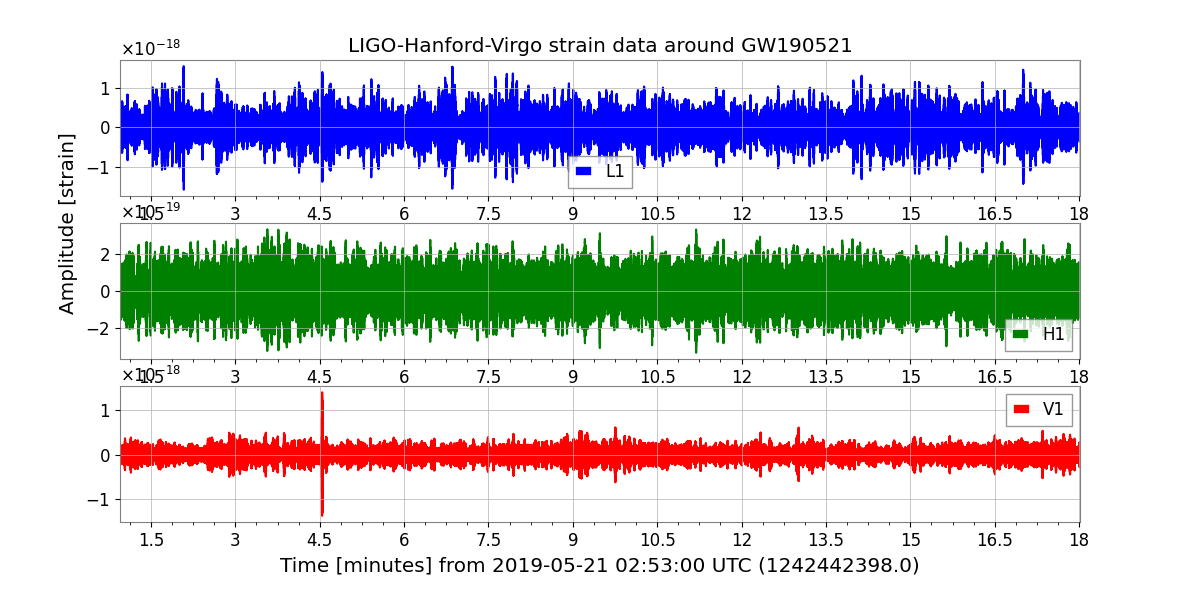
\includegraphics[width=0.6\textwidth]{GWanalysisProject_codefile/strainplot/GW190521strain.png}
            \caption{Strain data , with respect to time, recorded by each detector L1, H1 and V1 around GW190521}
            \label{fig:GW190521strain}
\end{figure}

\begin{figure}[htb]
    \centering
    \begin{subfigure}{0.45\textwidth}
       \centering
    
      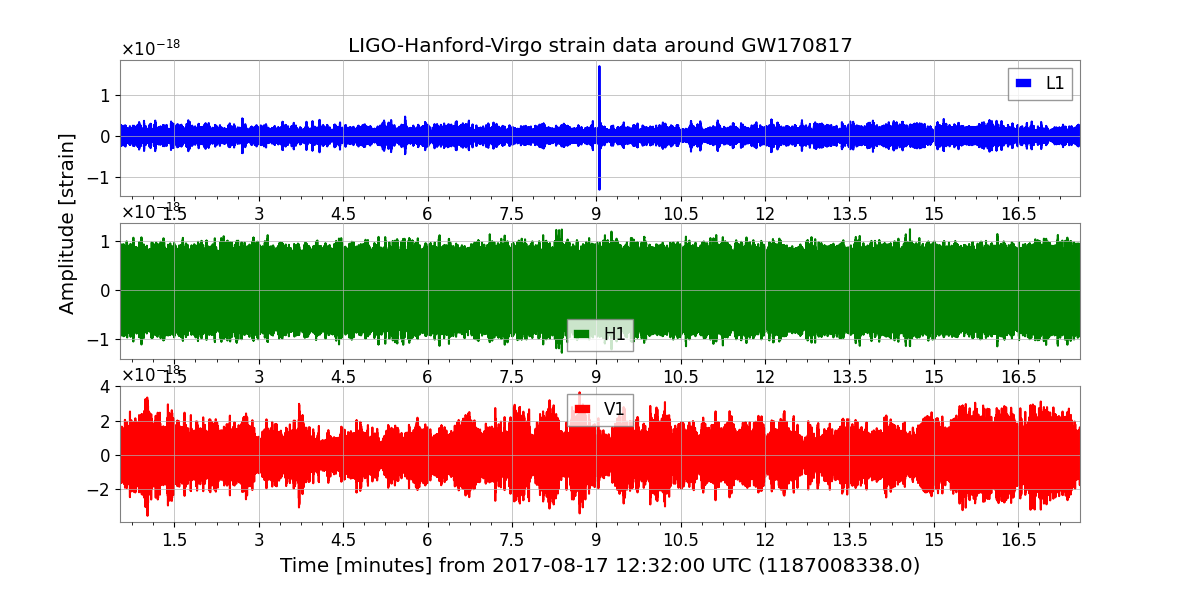
\includegraphics[width=1.27\linewidth]{GWanalysisProject_codefile/strainplot/GW170817strain.png}
           \caption{Strain data of GW170817}
           \label{fig: gw170817strain}
    \end{subfigure}
    % \hfill
    \begin{subfigure}{0.45\textwidth}
        \centering
        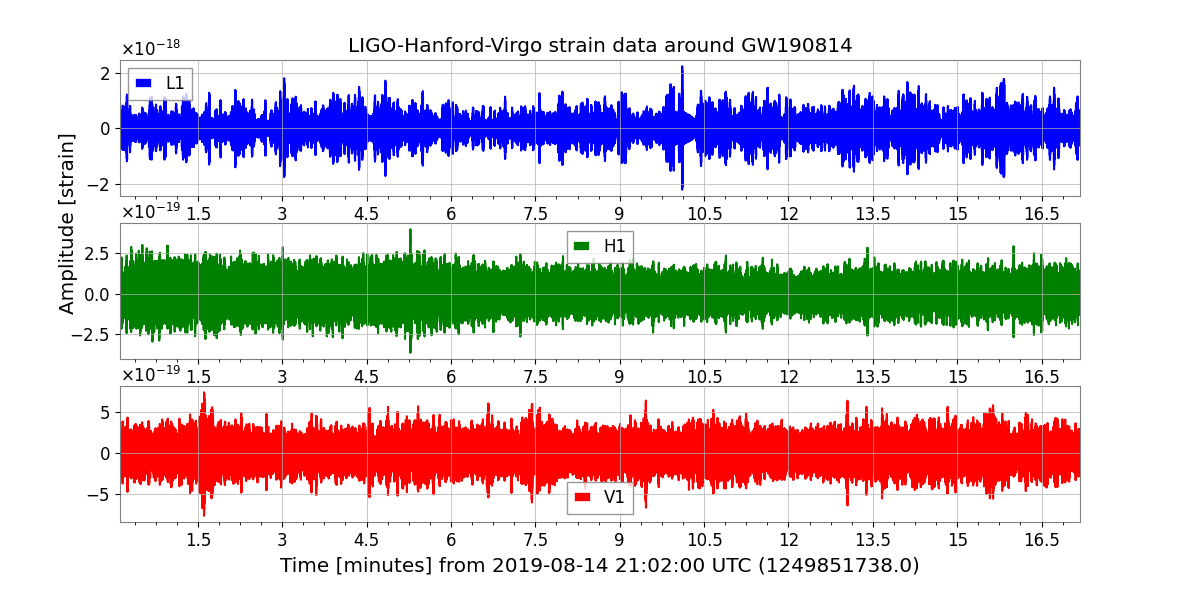
\includegraphics[width=1.27\linewidth]{GWanalysisProject_codefile/strainplot/GW190814strain.png}
        \caption{Strain data of GW190814}
        \label{fig: gw190521strain}
    \end{subfigure}
    \caption{Strain data , with respect to time, recorded by each detector L1, H1 and V1 around GW170817 and GW190814}
    \label{fig: strainplot}
\end{figure}

% start from here for description of asd plot
Important information on the noise properties of each instrument is provided by the Amplitude Spectral Density plot of the gravitational wave event, as observed by the LIGO-Livingston, LIGO-Hanford, and VIRGO detectors. 

\begin{figure}[htb]
    \centering
    \begin{subfigure}{0.45\textwidth}
       \centering
       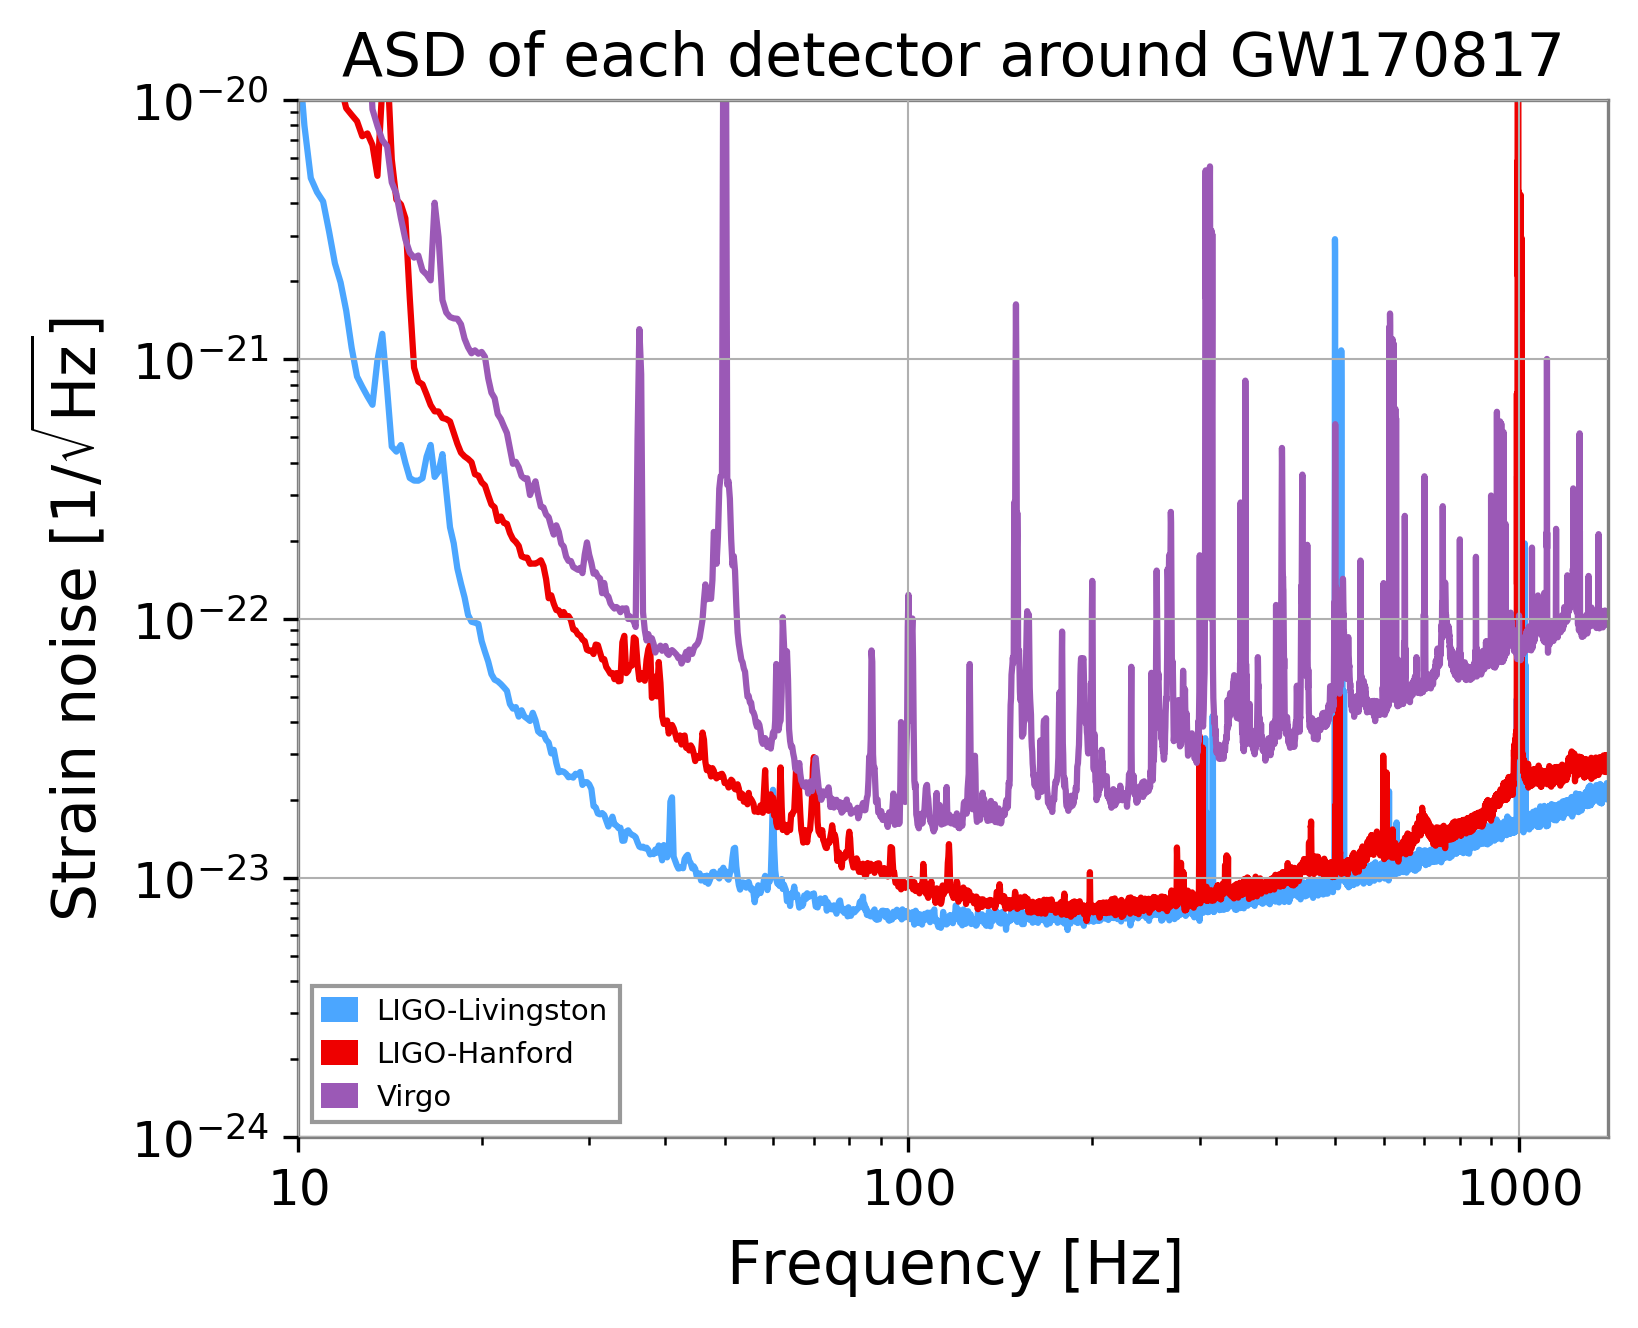
\includegraphics[width=1.0\linewidth]{GWanalysisProject_codefile/asd_plot/GW170817asd.png}
       \label{fig: gw170817asd}
    \end{subfigure}
    \hfill
    \begin{subfigure}{0.45\textwidth}
        \centering
        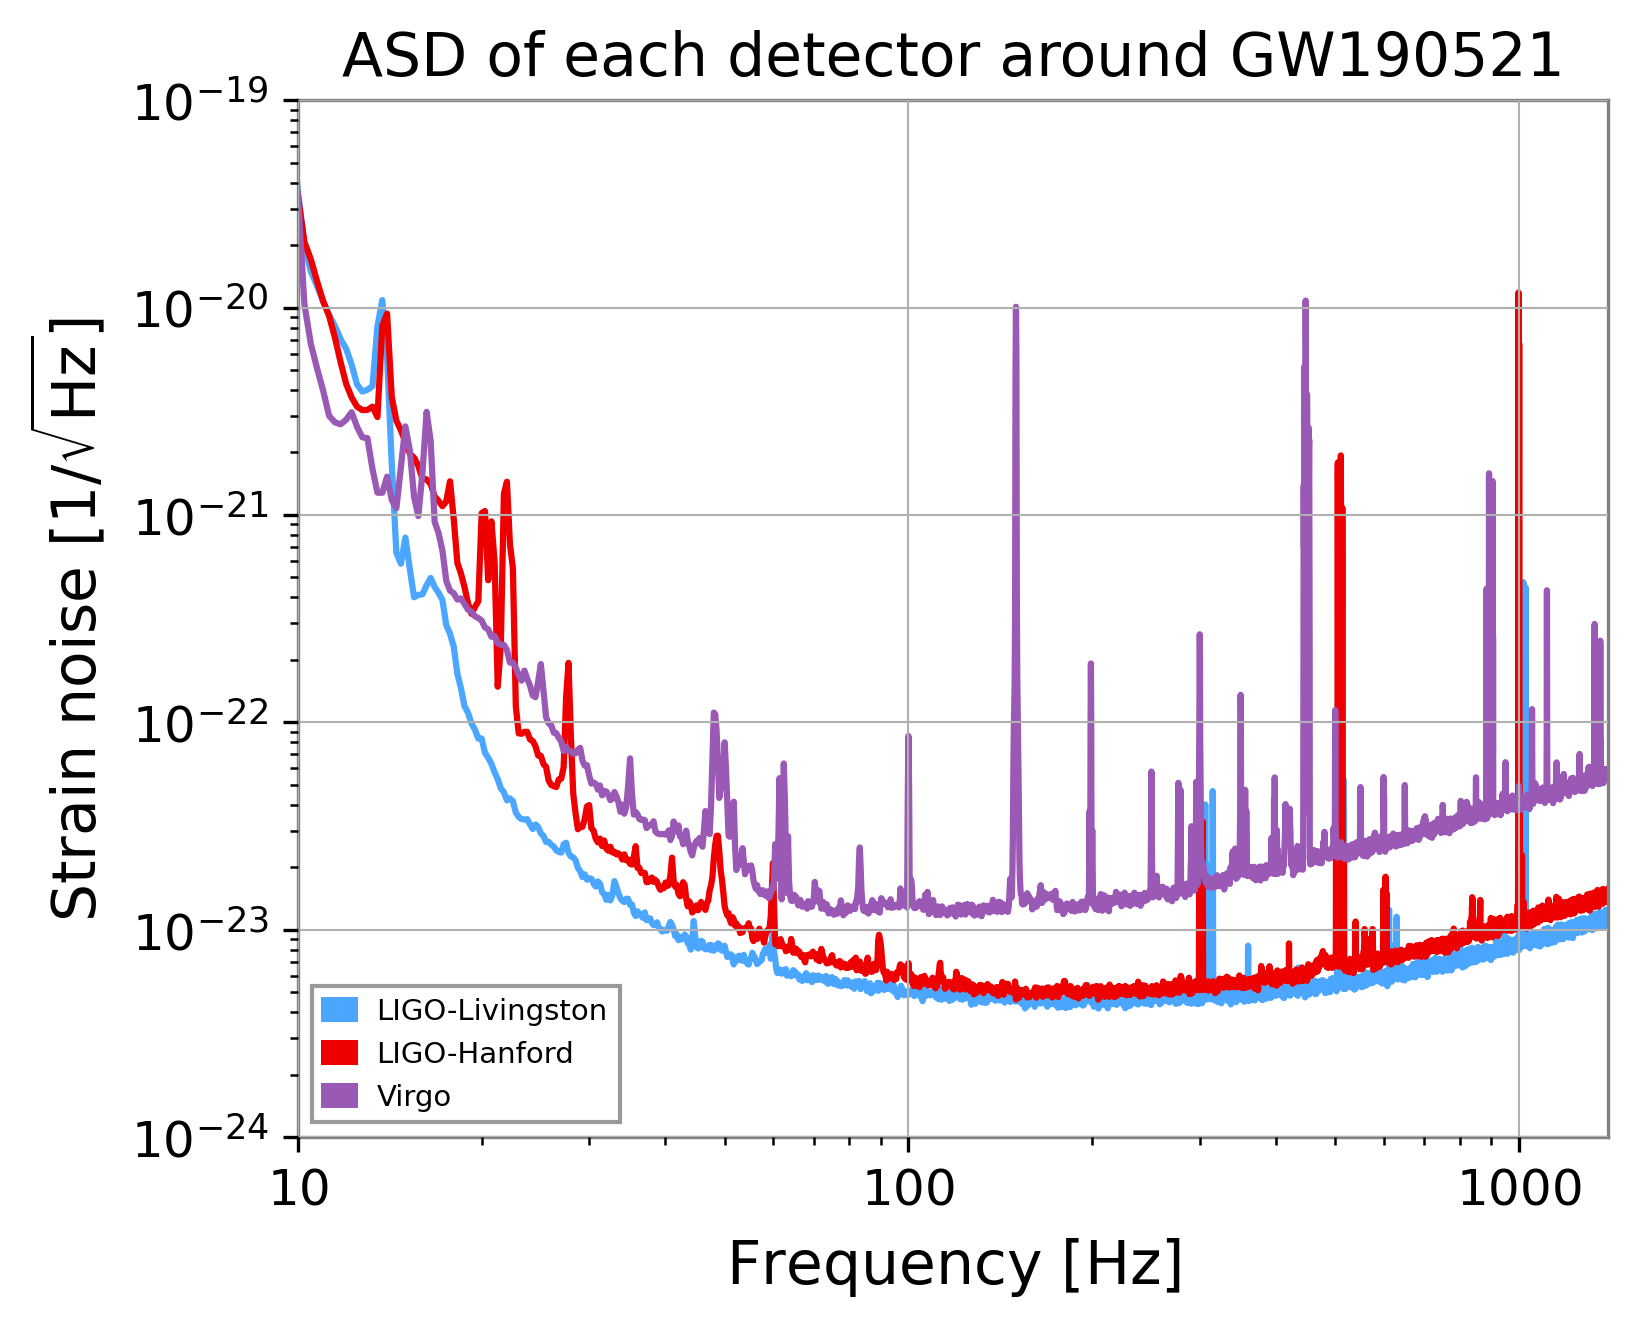
\includegraphics[width=1.0\linewidth]{GWanalysisProject_codefile/asd_plot/GW190521asd.png}
        \label{fig: gw190814asd}
    \end{subfigure}
    \hfill
    \begin{subfigure}{0.45\textwidth}
        \centering
        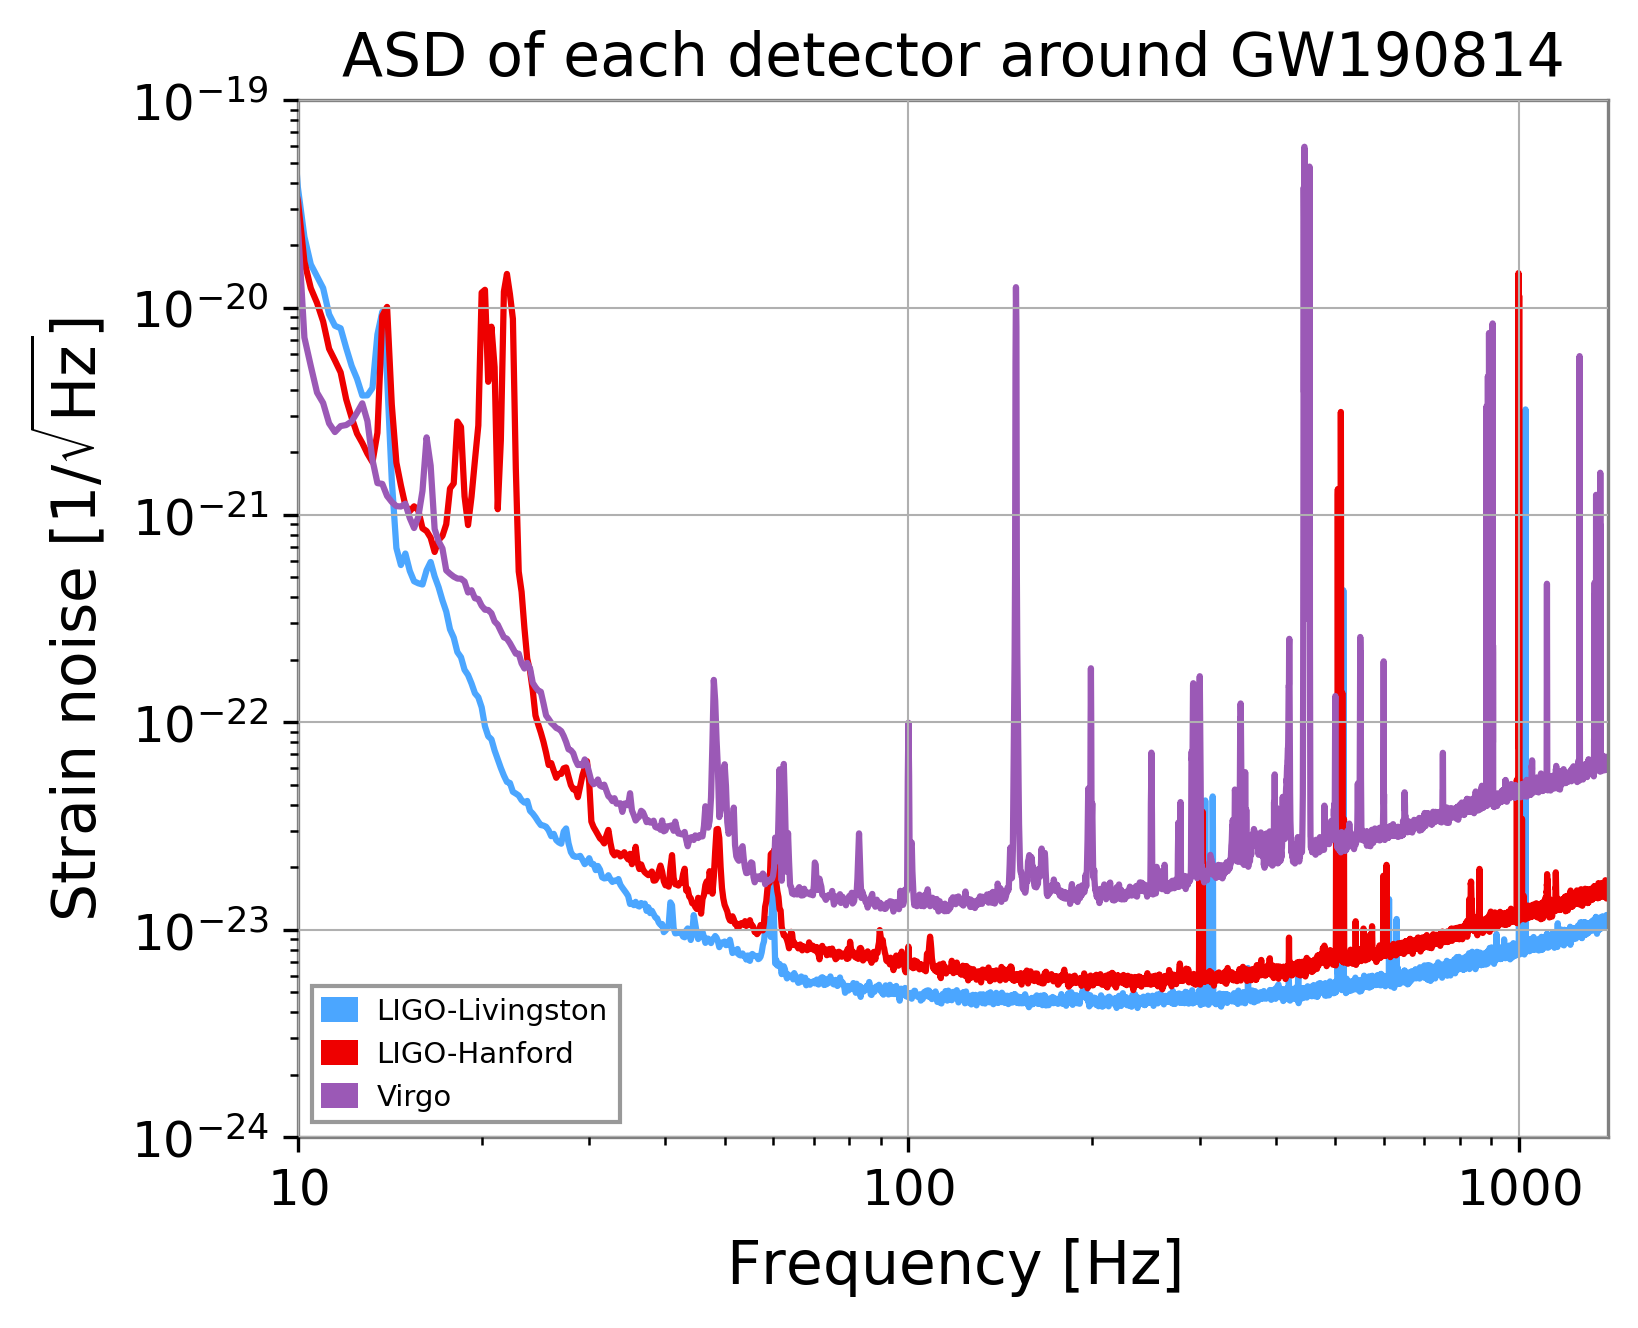
\includegraphics[width=1.0\linewidth]{GWanalysisProject_codefile/asd_plot/GW190814asd.png}
        \label{fig: gw190521asd}
    \end{subfigure}
    \caption{Amplitude Spectral Density (ASD) of each detector around GW170817, GW190521 and GW190814}
    \label{fig: asdplot}
\end{figure}

The Amplitude Spectral Density graphs of the LIGO and VIRGO detectors during the occurrences of GW170817, GW190814, and GW190521 offer significant insights into the detectors' sensitivity. In the case of GW170817, the LIGO-Livingston detector displayed the lowest strain noise over a wide range of frequencies, indicating superior sensitivity. The LIGO-Hanford detector, on the other hand, reported somewhat greater levels of noise. Above 100 Hz, the VIRGO detector exhibited the maximum level of strain noise, as seen by the purple curve. At lower frequencies (10-100 Hz), the level of strain noise reduced as the frequency increased, mostly because of the presence of seismic and ambient noise. At around 100 Hz, all detectors reached their maximum sensitivity with little strain noise, which subsequently rose at higher frequencies (100-1000 Hz) as a result of thermal and quantum noise.

Similarly, in the cases of the GW190814 and GW190521 events, the LIGO-Livingston detector consistently exhibited the highest sensitivity with the lowest level of strain noise. It was followed by the LIGO-Hanford detector, while the VIRGO detector had the highest level of strain noise. The VIRGO detector displayed many distinct peaks at various frequencies, suggesting the presence of narrowband noise sources or resonances. 


\begin{figure}[htb]
    \centering
    \begin{subfigure}{0.45\textwidth}
       \centering
       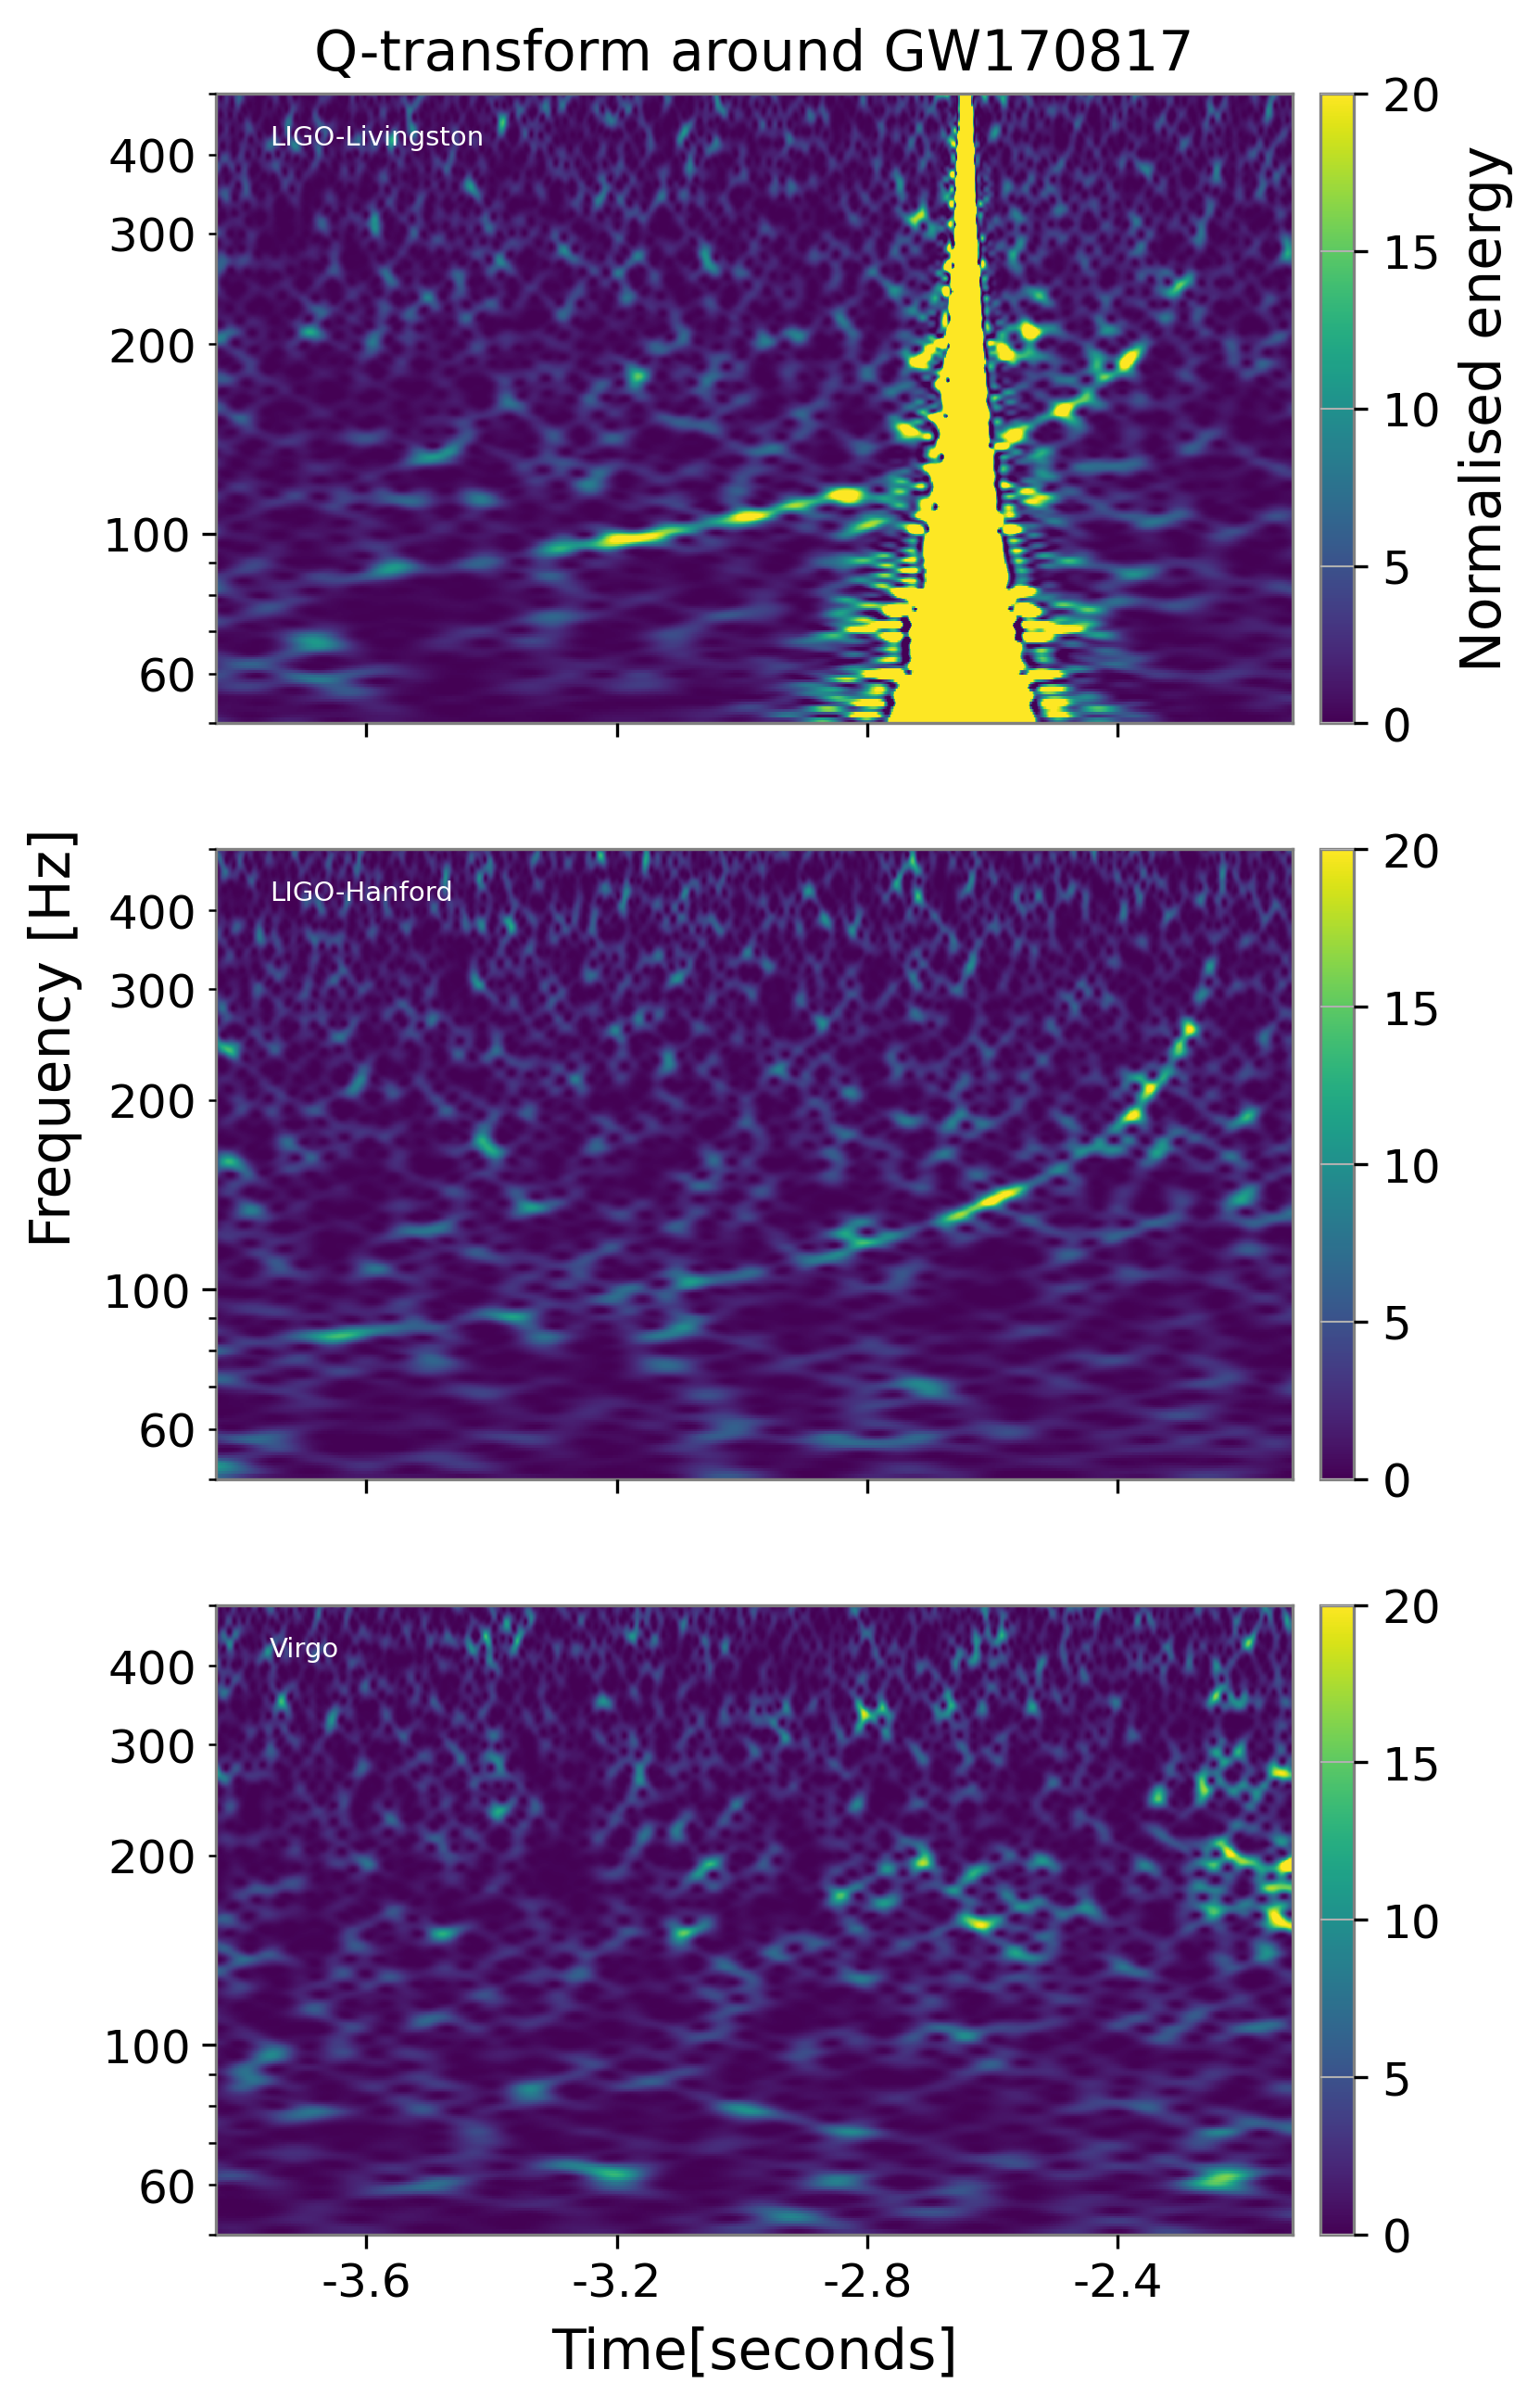
\includegraphics[width=0.65\linewidth]{GWanalysisProject_codefile/qtransformplot/GW170817_qtransform.png}
       \label{fig: gw170817qtransform}
    \end{subfigure}
    \hfill
    \begin{subfigure}{0.45\textwidth}
        \centering
        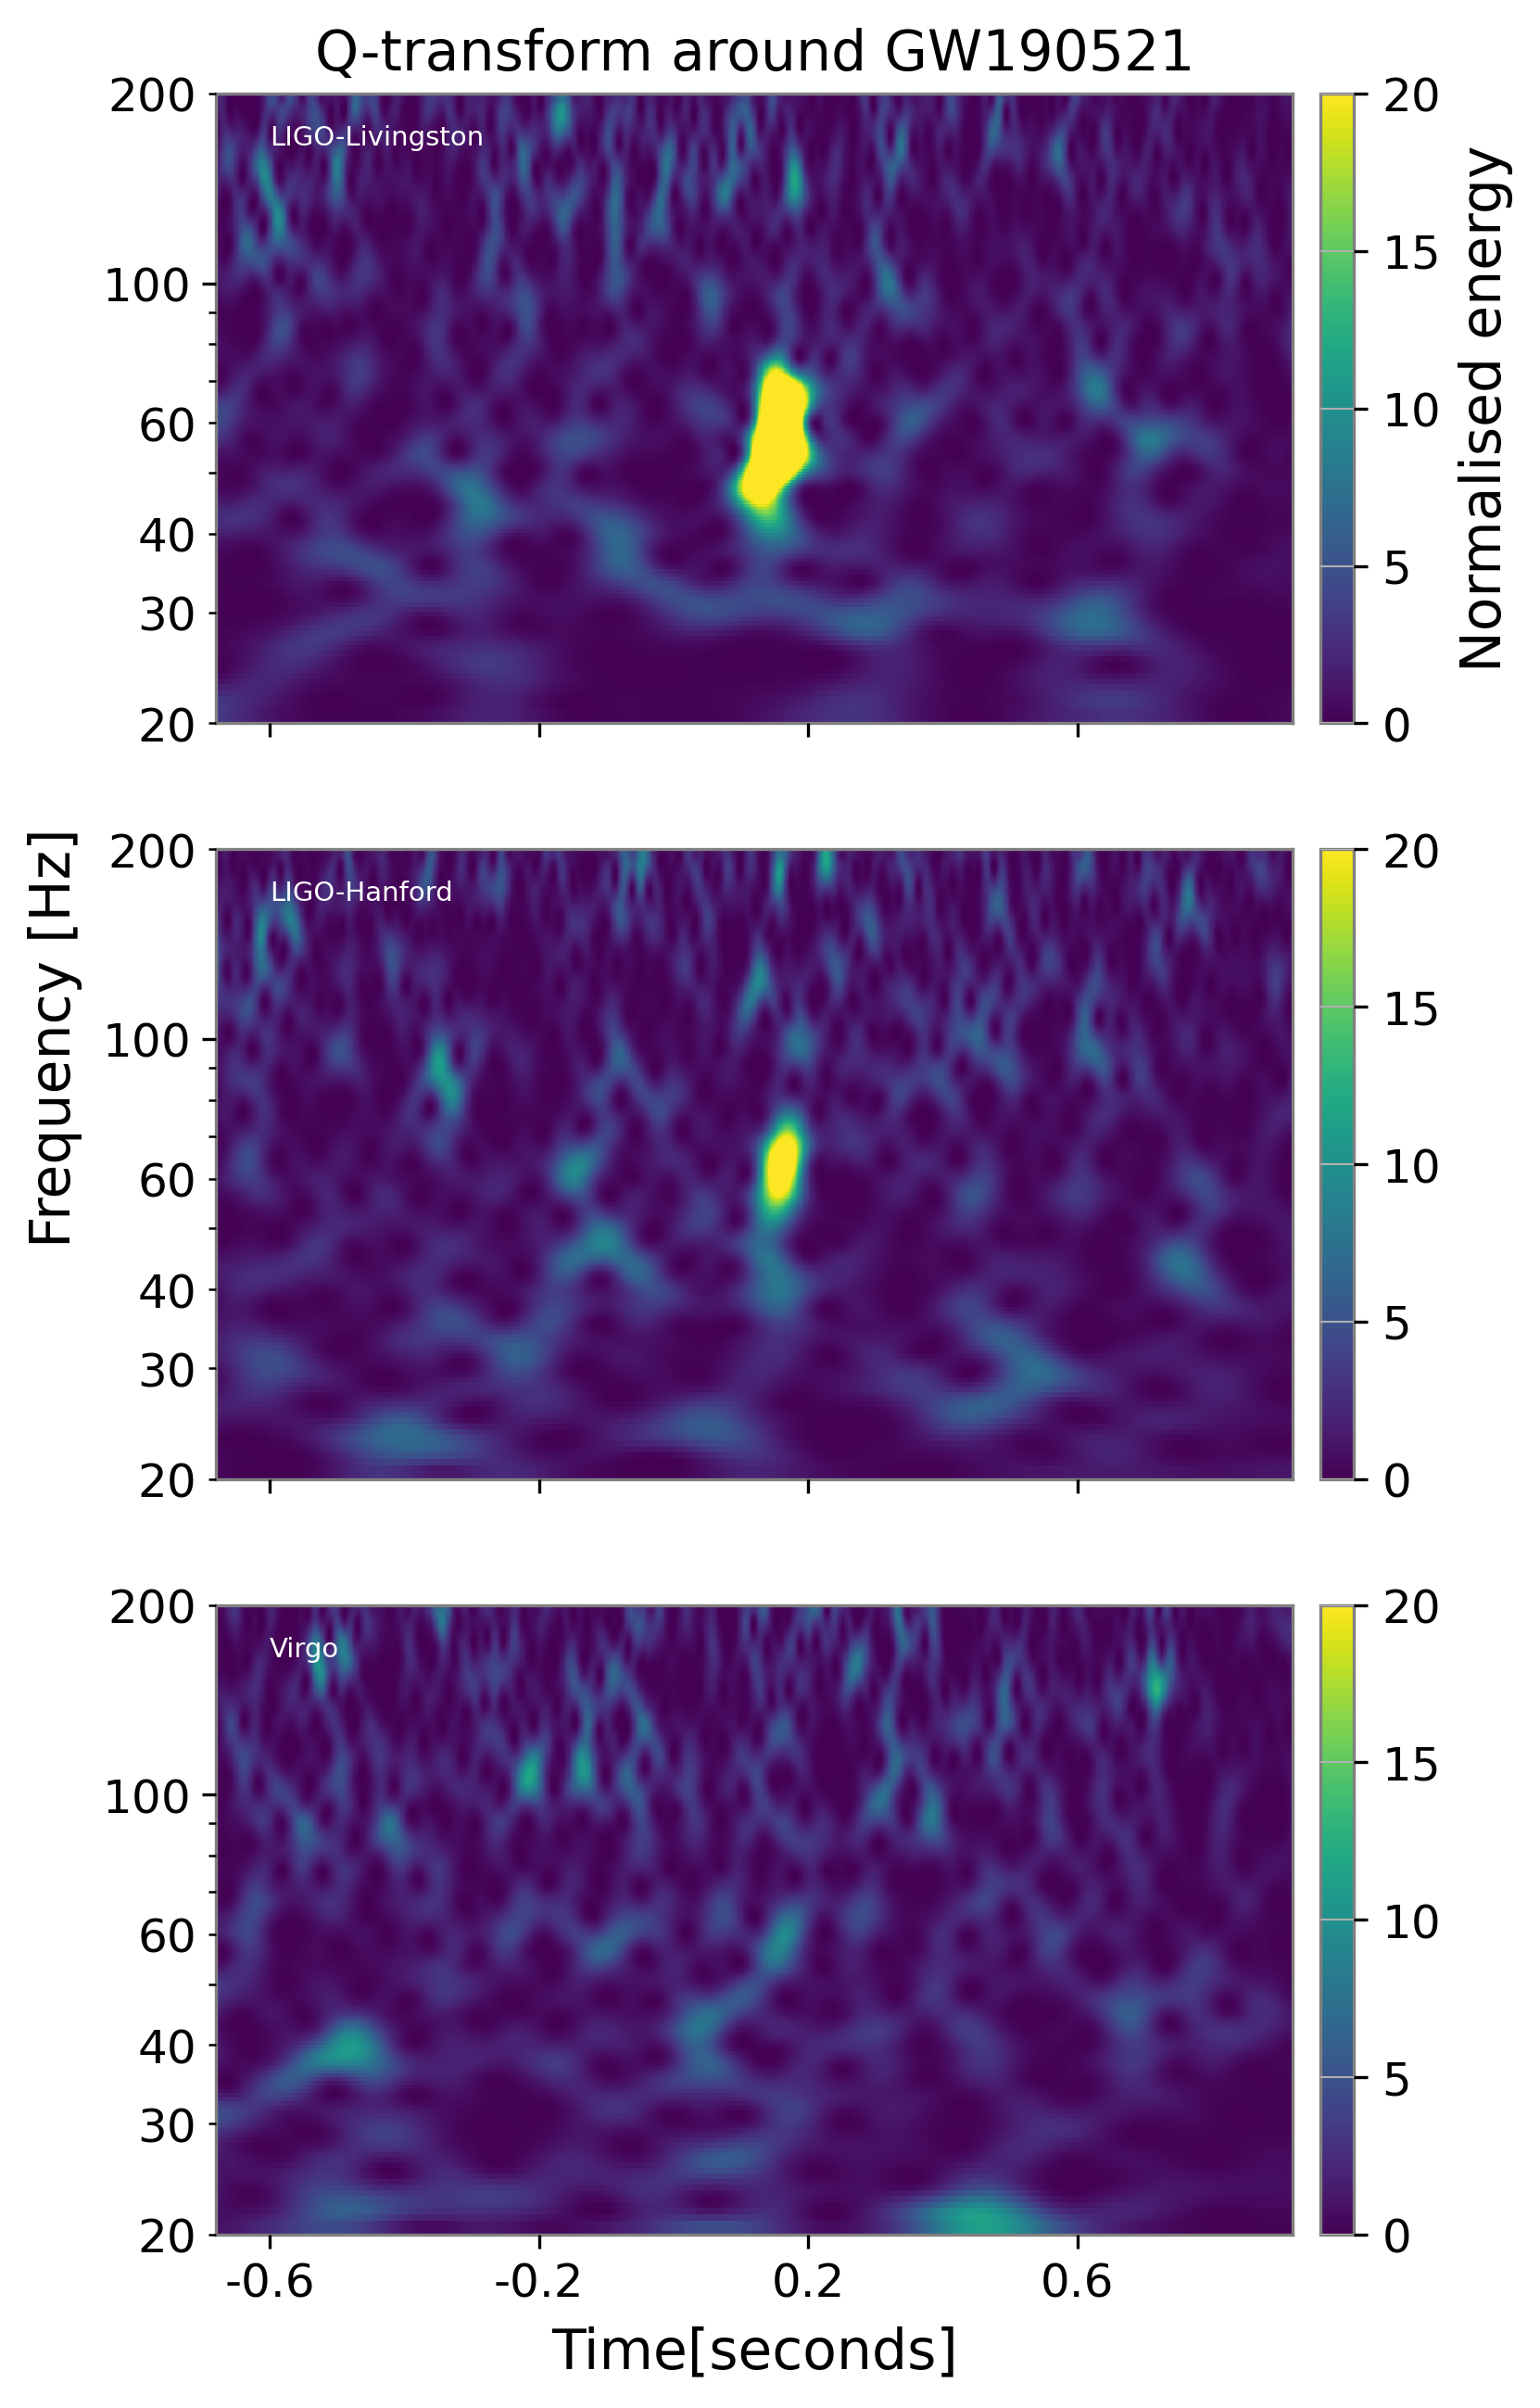
\includegraphics[width=0.65\linewidth]{GWanalysisProject_codefile/qtransformplot/GW190521_qtransform.png}
        \label{fig: gw190814qtransform}
    \end{subfigure}
    \hfill
    \begin{subfigure}{0.45\textwidth}
        \centering
        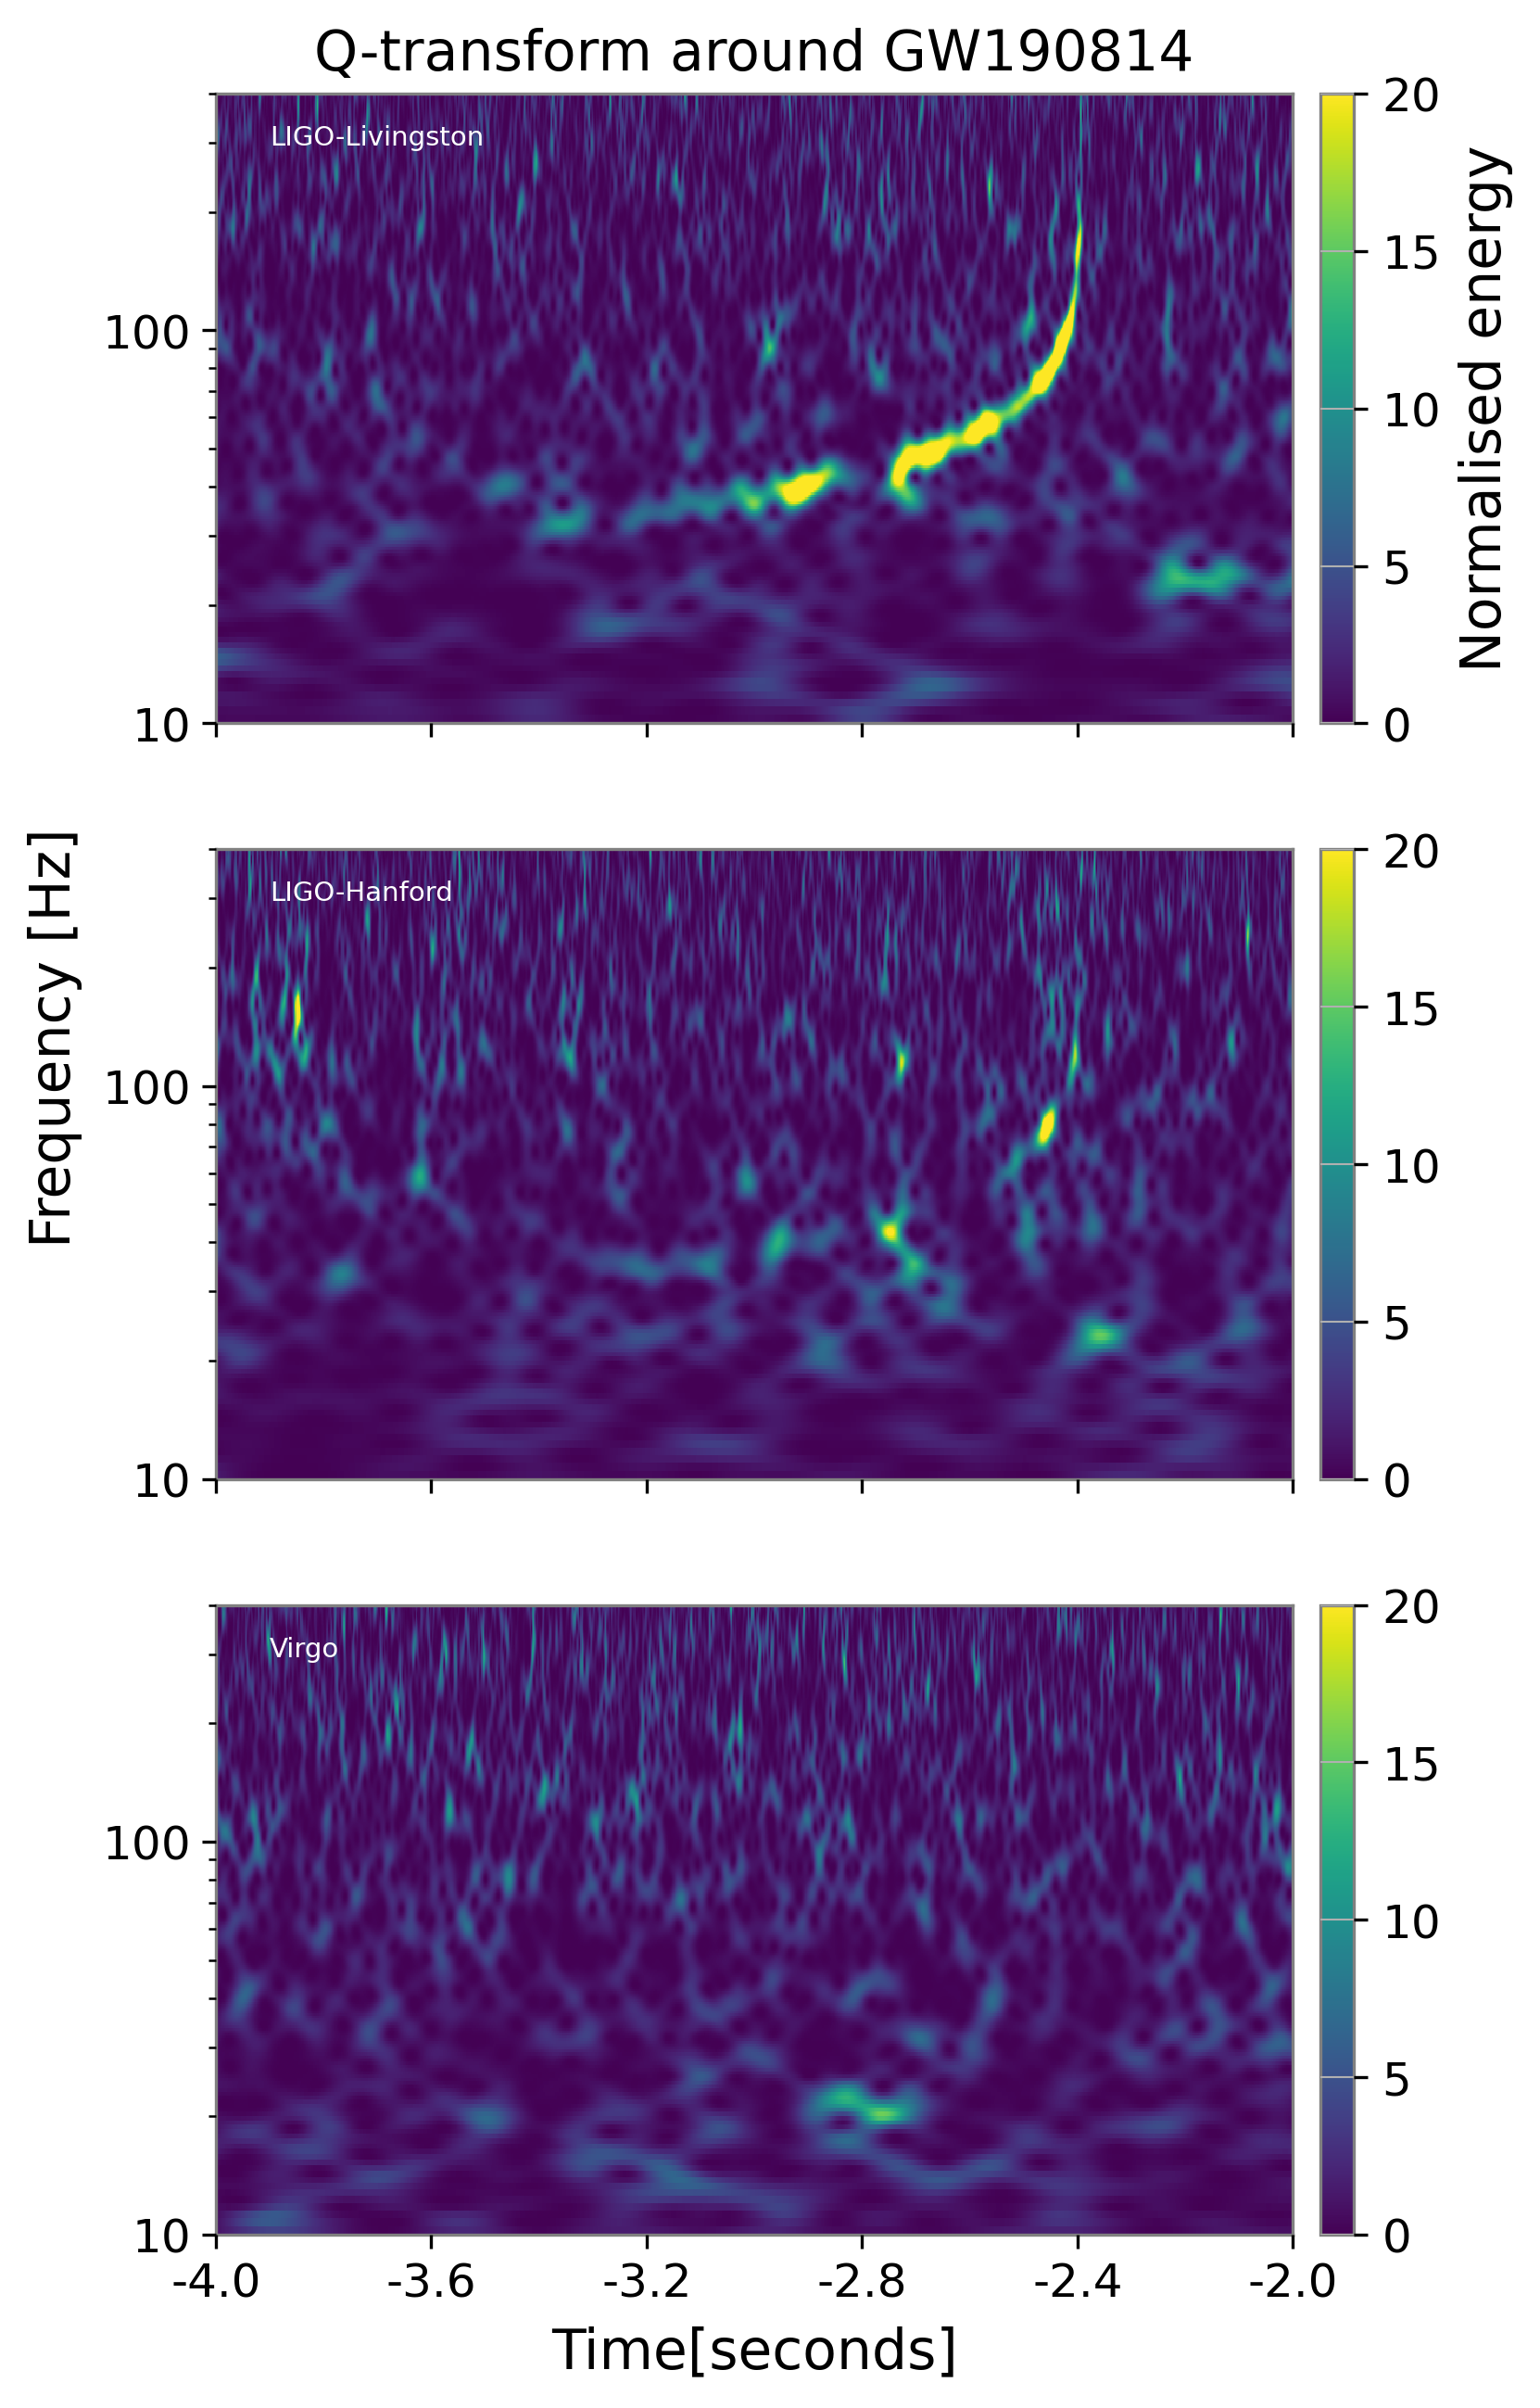
\includegraphics[width=0.65\linewidth]{GWanalysisProject_codefile/qtransformplot/GW190814_qtransform.png}
        \label{fig: gw190521qtransform}
    \end{subfigure}
    \caption{Amplitude Spectral Density of each detector around GW170817, GW190521 and GW190814}
    \label{fig: qtransformplot}
\end{figure}

Figure [\ref{fig: qtransformplot}] depicted a two-dimensional spectrogram of the data, illustrating the variations in strength of the gravity waves at different frequencies during the event. 
The spectrograms of GW170817 exhibit a distinct chirp signal, with the most notable instance detected in the LIGO-Livingston data. The chirp signal may be observed as a vivid yellow streak, starting at a frequency of around 60 Hz and quickly rising to over 300 Hz as the event moves closer to the merger. The increase in both the frequency and amplitude of the signal corresponds to the last phase of the binary neutron stars' approach towards each other, ultimately resulting in their merger. However, the LIGO-Livingston spectrogram exhibits a loud glitch occurring during the time frame of -2.8 to -2.1 seconds. Nevertheless, the chirp signal of GW170817 remains apparent. A comparable chirp is observed in the LIGO-Hanford spectrogram. On the other hand, the VIRGO spectrogram shows diminished prominent characteristics. 

Similarly, The GW190521 event exhibits a concise, low-frequency signal, predominantly centered around 60 Hz, as detected by the LIGO-Livingston and LIGO-Hanford detectors. This signal is most likely caused by the substantial mass of the colliding black holes. This brief transient signal, lasting for only a fraction of a second just before the merging of two objects, emphasizes the swift and immediate process of the merger. The VIRGO detector detected a signal of lesser magnitude, in line with its reduced sensitivity.

Similarly, the GW190814 event exhibits a unique chirp signal, which is particularly evident in the LIGO-Livingston data. The signal begins at a low frequency and swiftly rises as the two objects spiral inward and combine, exhibiting the typical behavior of a black hole and a compact object coalescence. The Hanford and VIRGO detector captures a less intense signal.

\begin{figure}[h]
            \centering          
            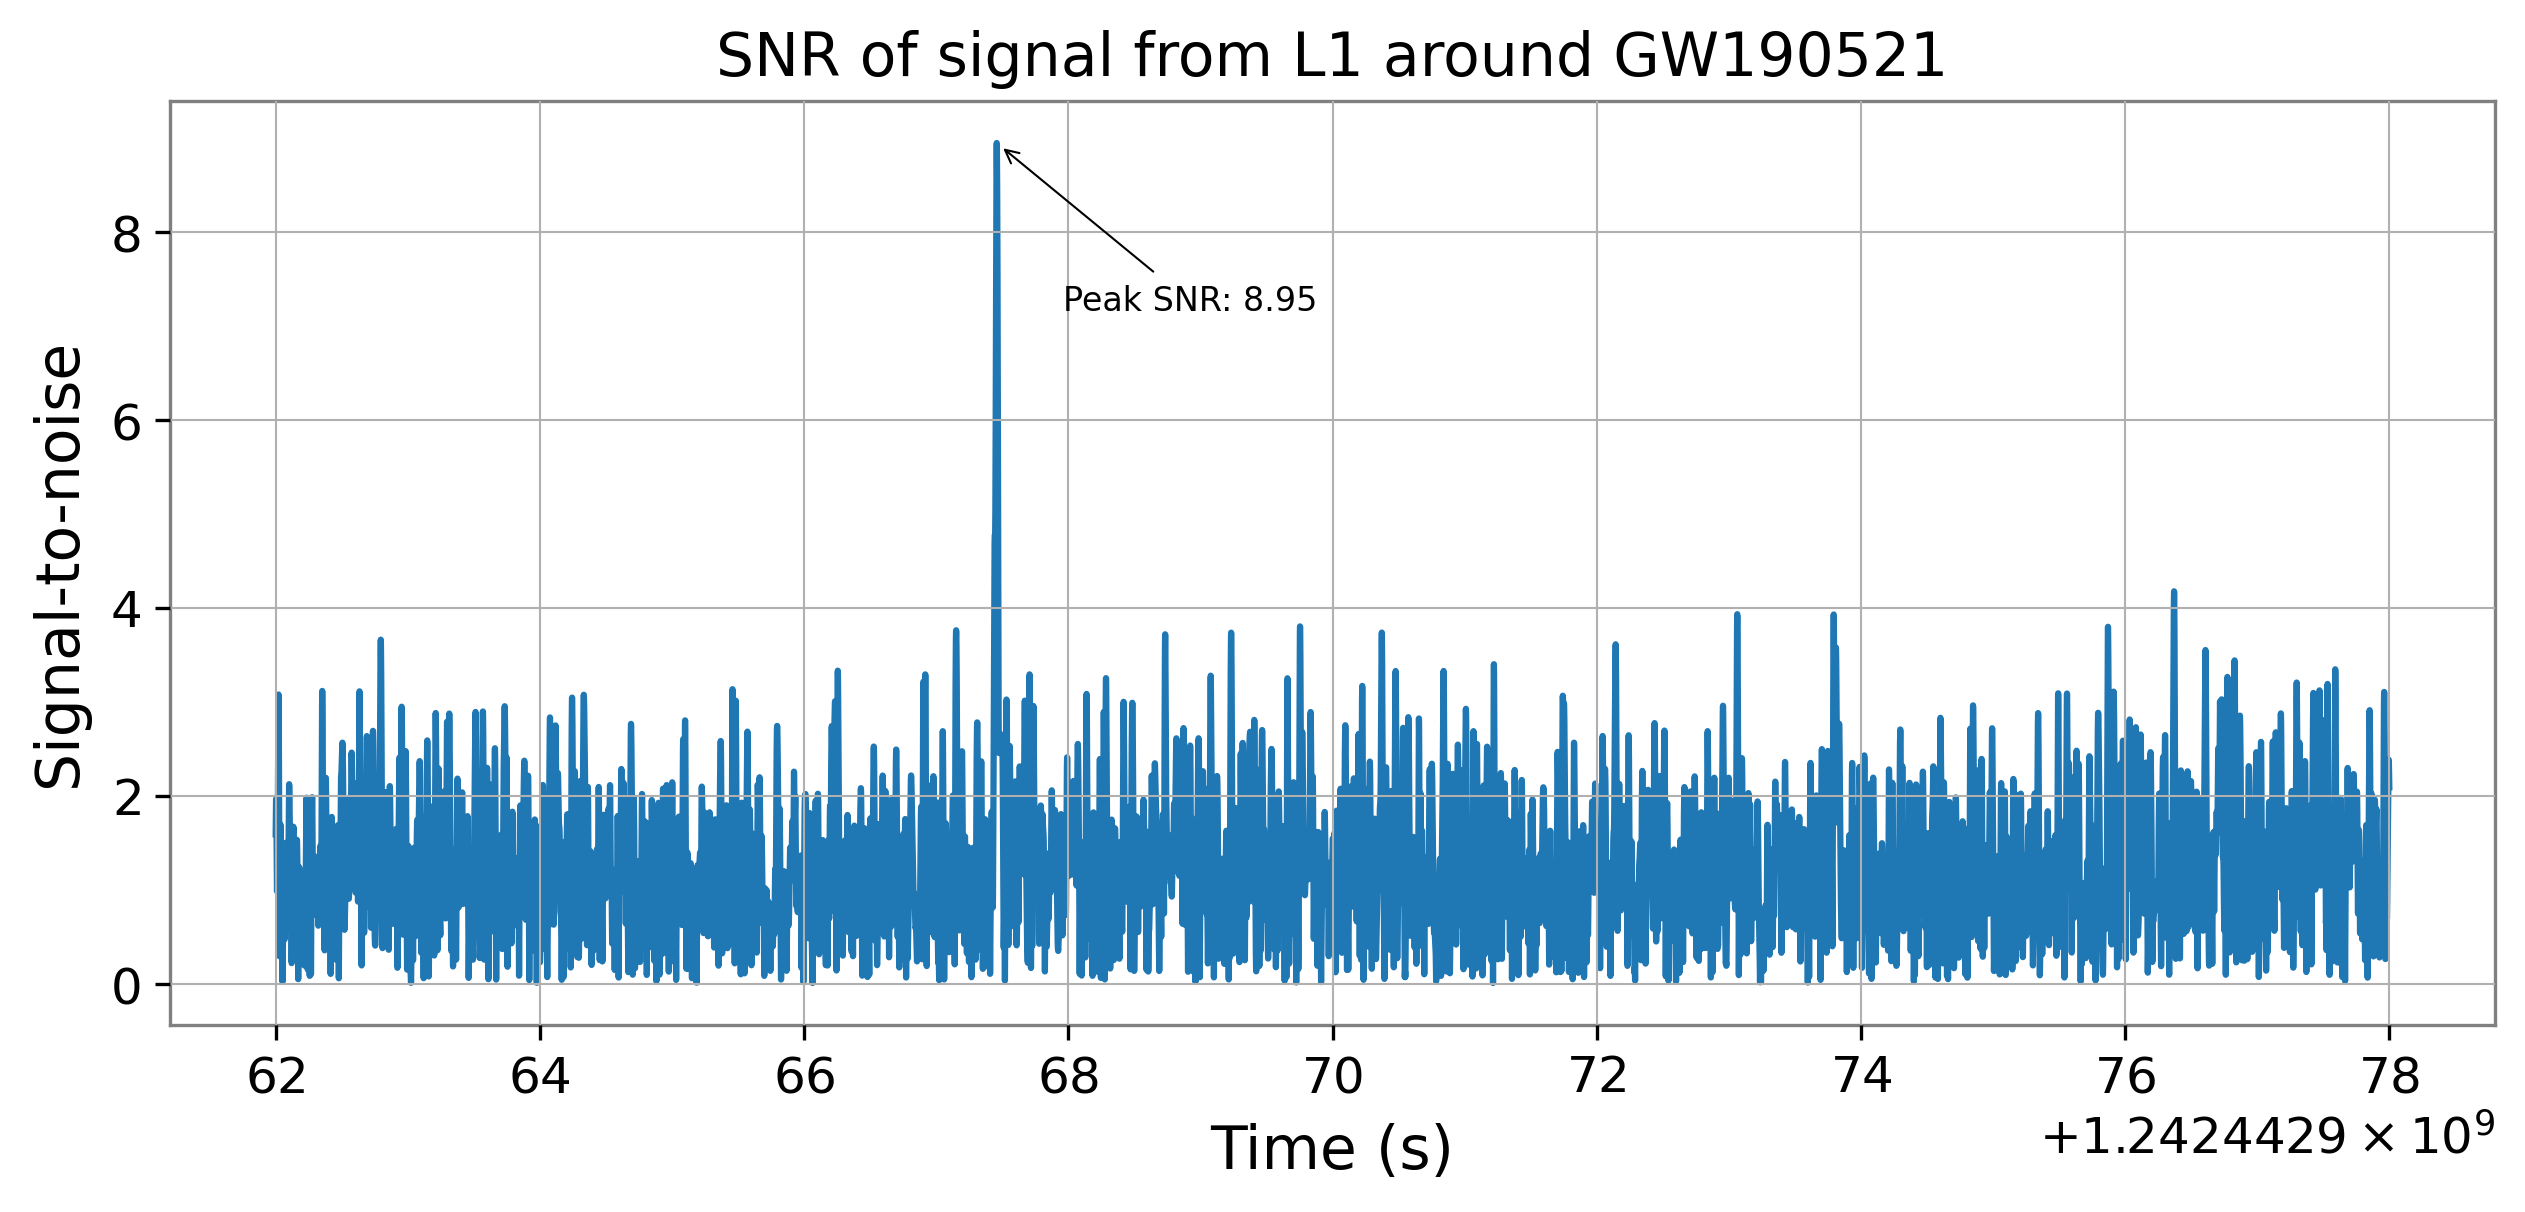
\includegraphics[width=0.85\textwidth]{GWanalysisProject_codefile/SNRplot/SNRL1GW190521.png}
            \caption{Signal to Noise Ratio around GW190521}
            \label{fig:GW190521SNR}
\end{figure}

\begin{figure}[h]
            \centering          
            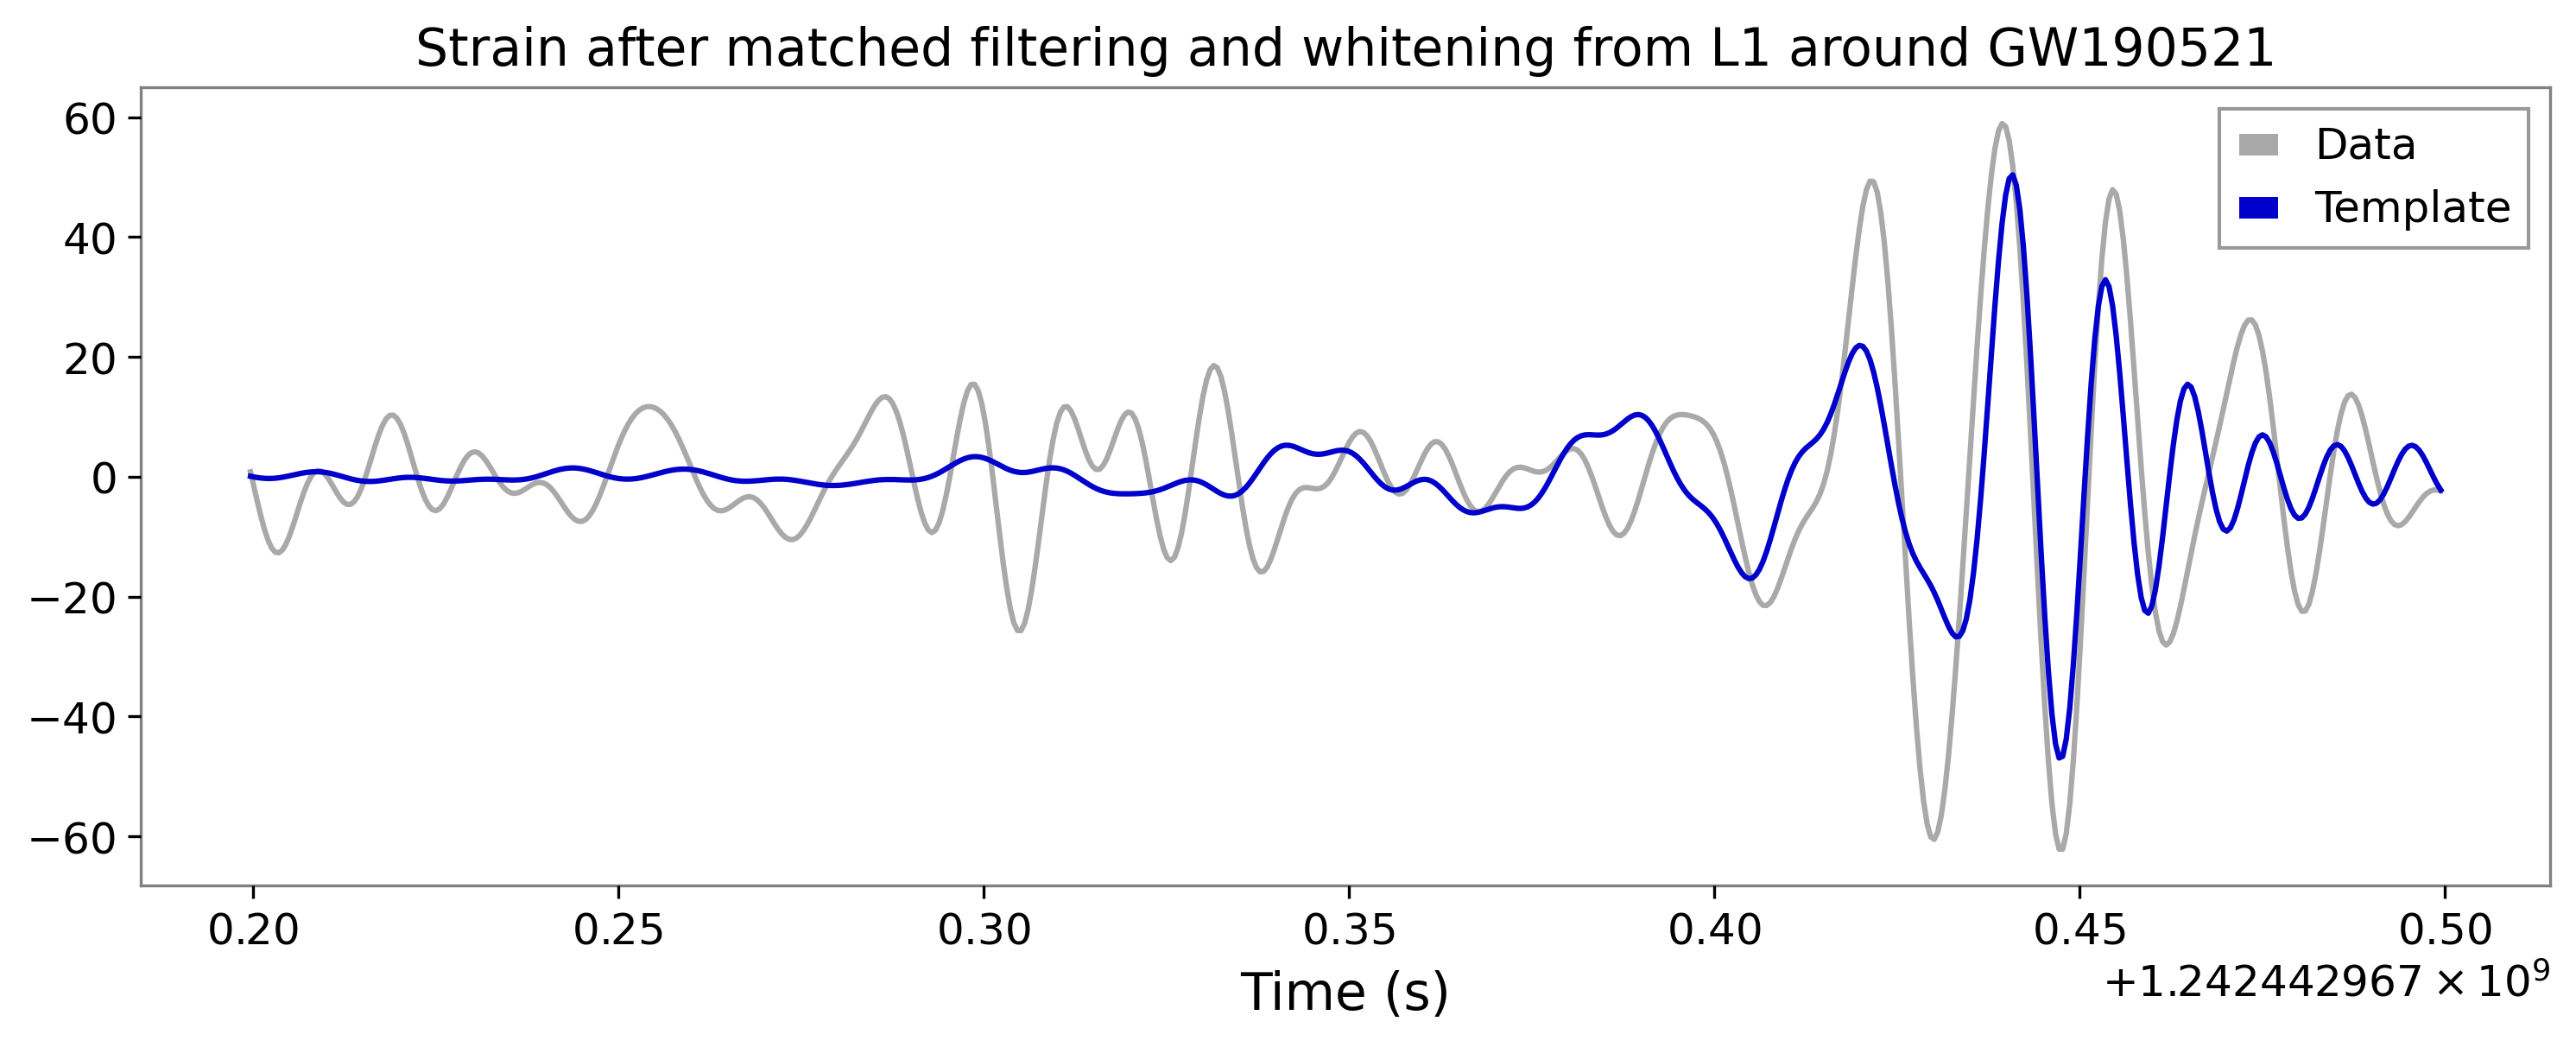
\includegraphics[width=0.85\textwidth]{GWanalysisProject_codefile/templateplot/templateL1GW190521.png}
            \caption{Whitened Template data calculated from numerical solution of GR and actual recorded data around GW190521}
            \label{fig:GW190521template}
\end{figure}


The Signal-to-Noise Ratio analysis was conducted on data from the L1 detector to identify the presence of a gravitational wave signal associated with the event GW190521. The signal-to-noise ratio measures the signal's intensity compared to the background noise, serving as a tool to evaluate the probability of a true gravitational wave signal being present in the observed data.

The SNR is graphed against time in figure \ref{fig:GW190521SNR}, with the time axis centered on the anticipated event time. The analysis showed a significant peak in the signal-to-noise ratio of 8.95 at around 68 seconds. The amplitude of this peak is considerably greater than the background noise, suggesting a robust detection of the signal.

% \begin{figure}[h]
%             \centering          
%             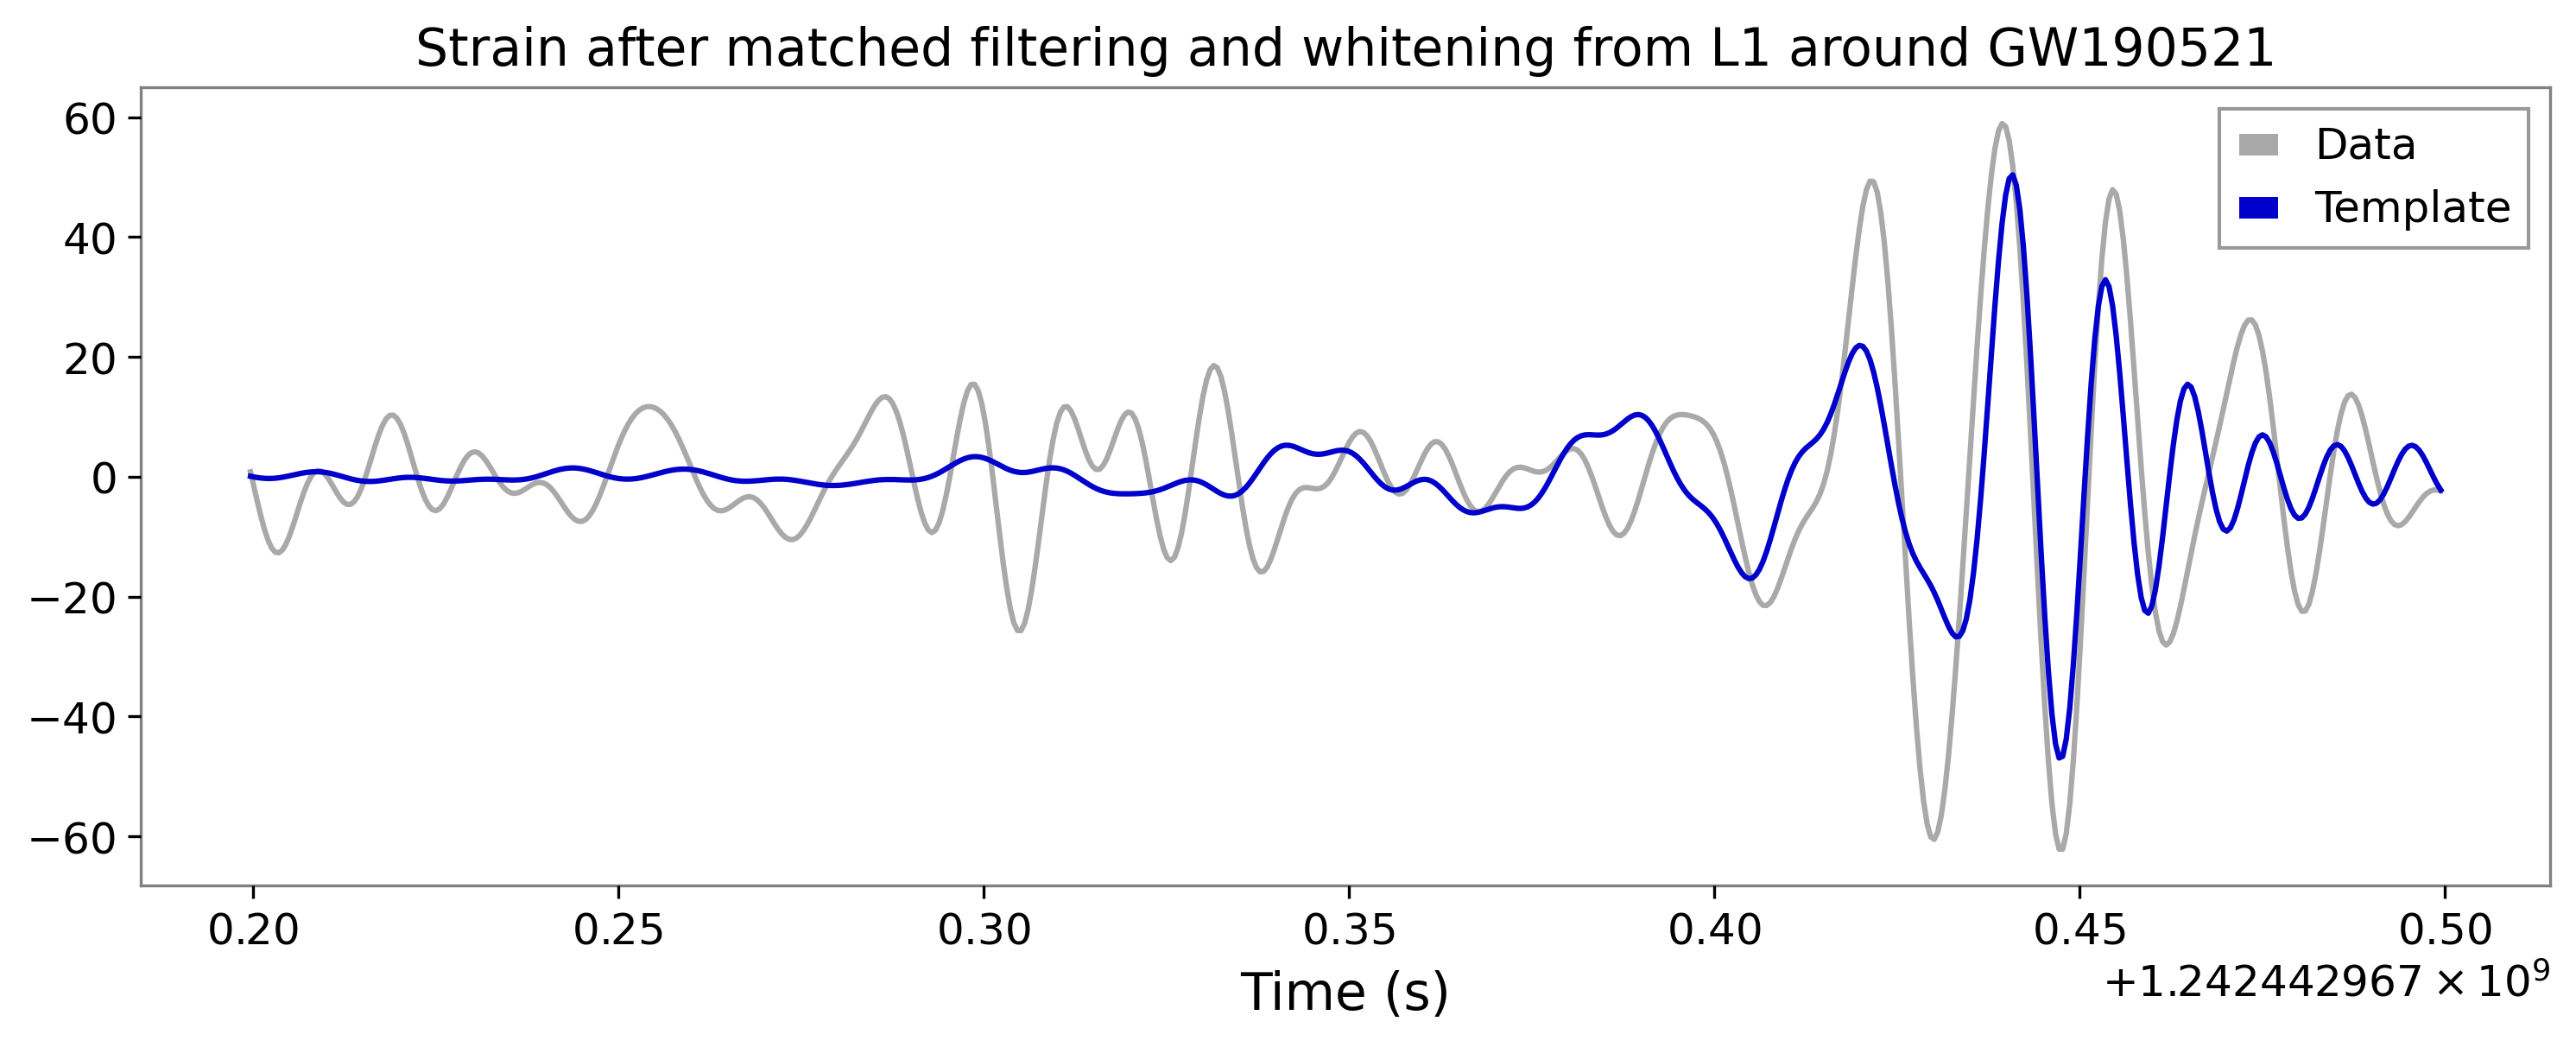
\includegraphics[width=0.95\textwidth]{GWanalysisProject_codefile/templateplot/templateL1GW190521.png}
%             \caption{Whitened Template data calculated from numerical solution of GR and actual recorded data around GW190521}
%             \label{fig:GW190521template}
% \end{figure}

We then generated a template plot by employing \texttt{get\_td\_waveform} function from the \texttt{pycbc.wa\\veform} module. Specifically, I used the waveform \texttt{approximant = 'IMRPhenomPv3HM'} (see Appendix \ref{code2}) with mass parameters of 90 and 65 $M_\odot$, and a distance of 4600 Mpc. The \texttt{'IMRPhen\\omPv3HM'} performs numerical solution of relativity of provided parameters. The waveform was computed with a time resolution of \texttt{conditioned.delta\_t} (see Appendix \ref{code2}) and a frequency lower bound of 20 Hz.
\begin{figure}[h]
            \centering          
            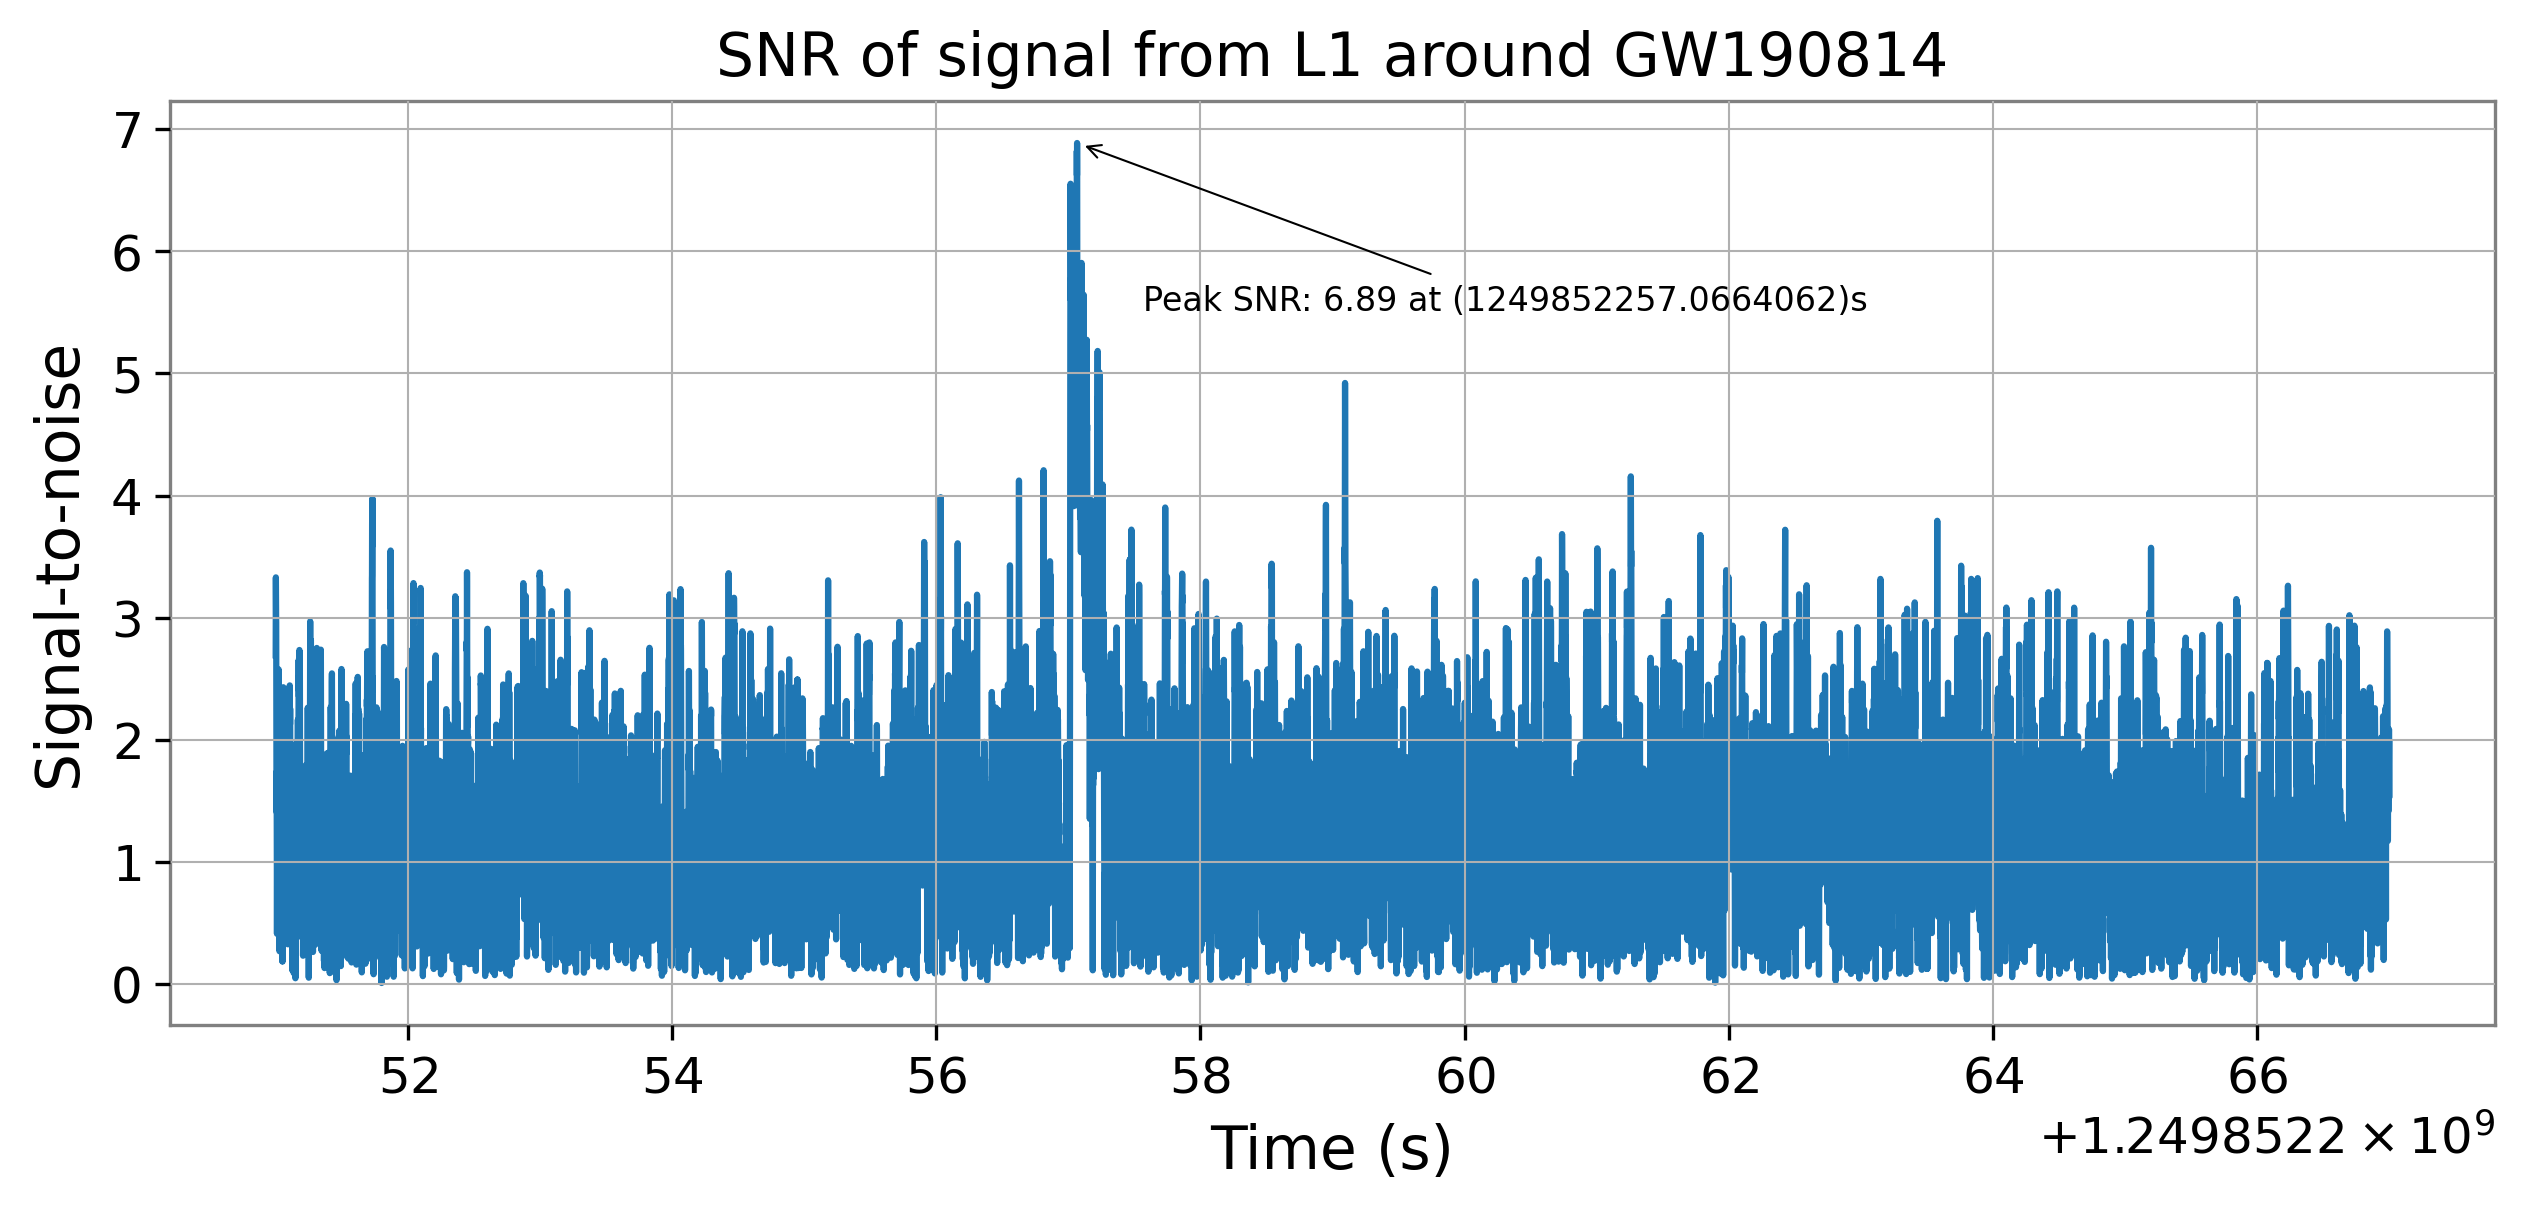
\includegraphics[width=0.78\textwidth]{GWanalysisProject_codefile/SNRplot/SNRL1GW190814.png}
            \caption{SNR from L1 detector around GW190814}
            \label{fig:GW190814SNR}
\end{figure}

\begin{figure}[h]
            \centering          
            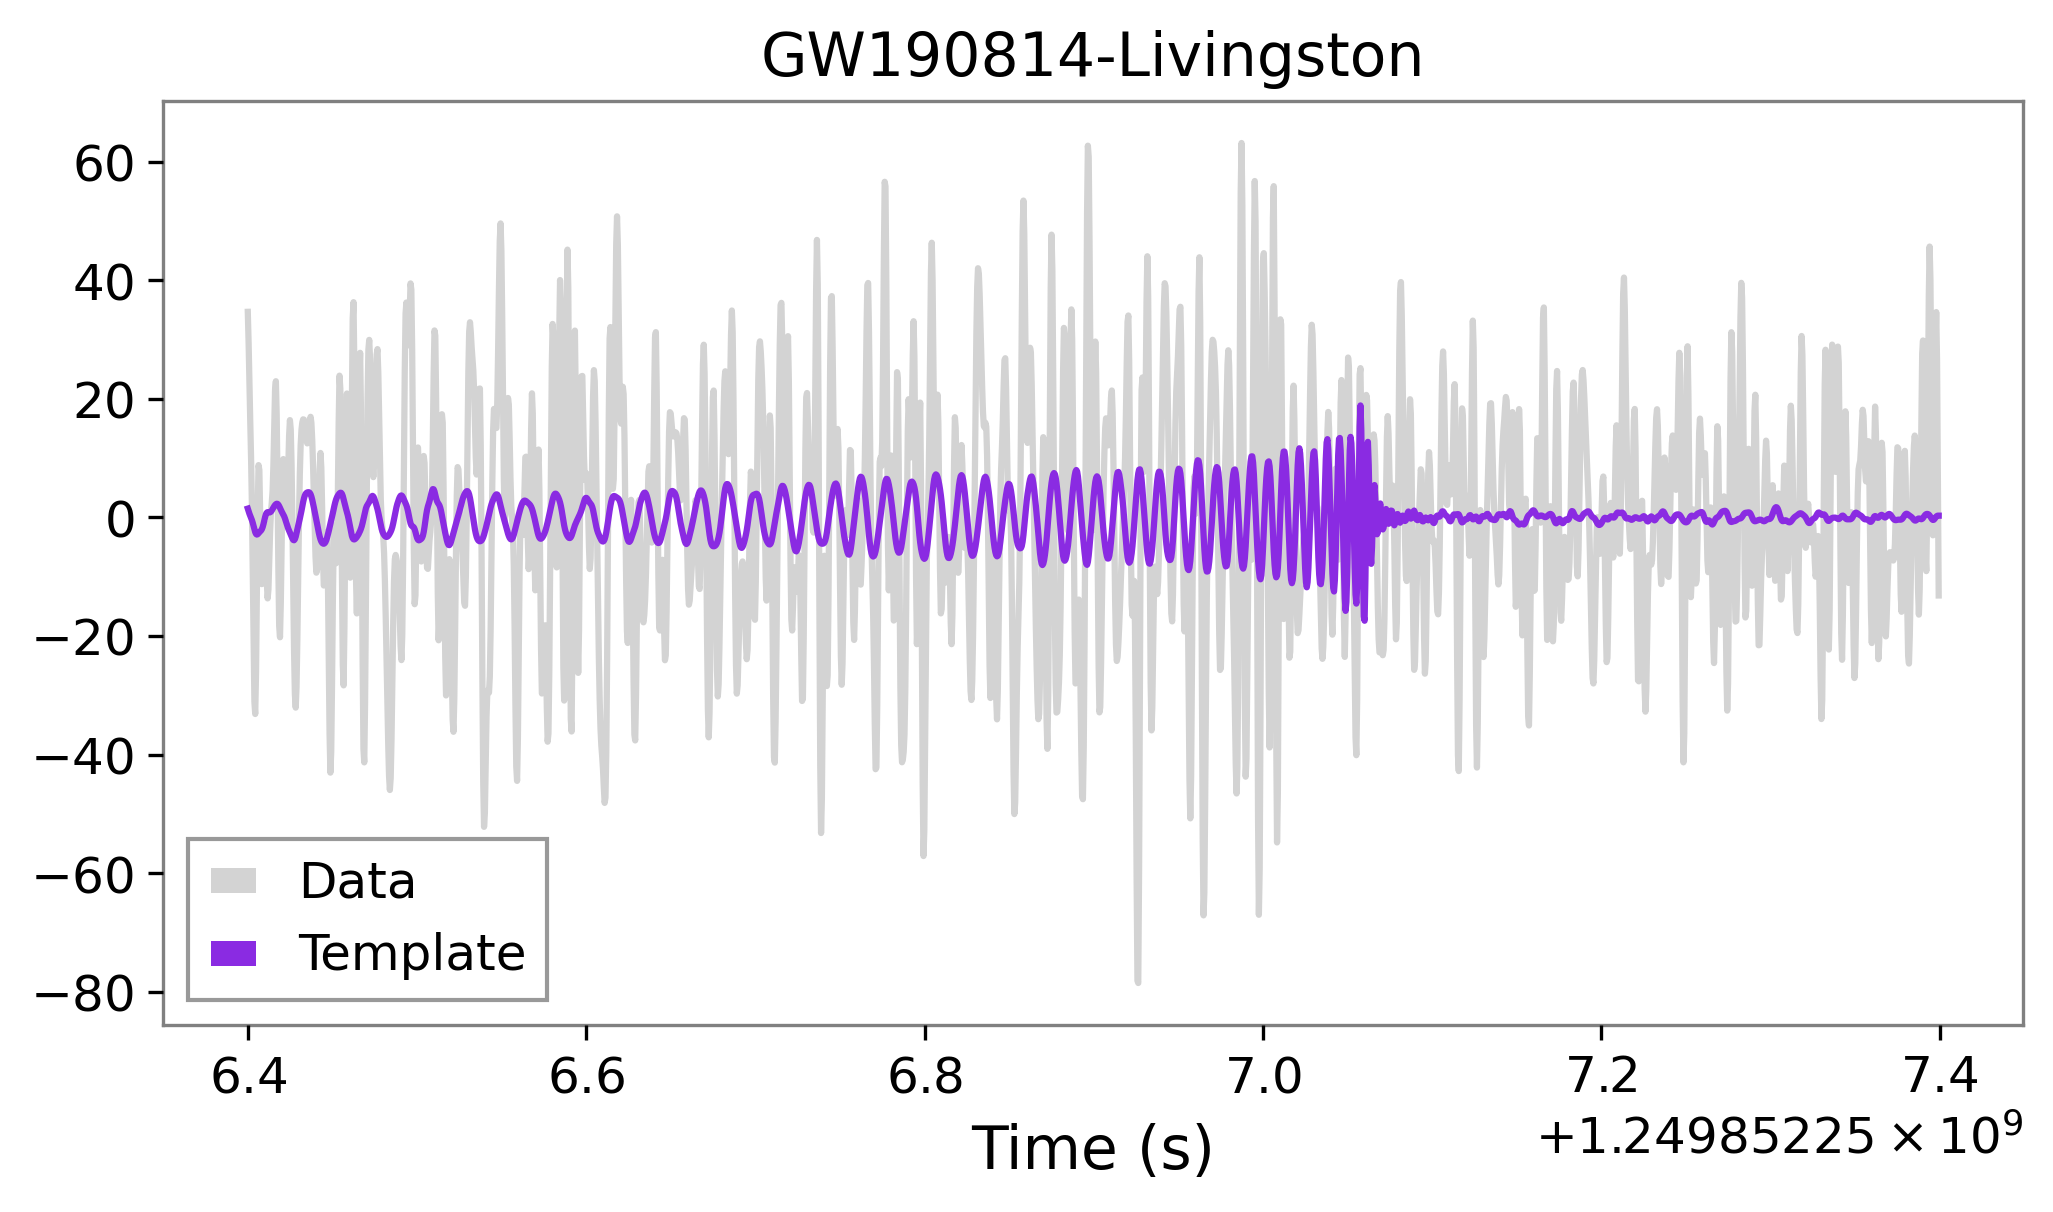
\includegraphics[width=0.75\textwidth]{GWanalysisProject_codefile/templateplot/templateL1GW190814.png}
            \caption{Whitened Template data calculated from numerical solution of GR and actual recorded data around GW190814}
            \label{fig:GW190814template}
\end{figure}

The result figure \ref{fig:GW190521template} shows the frequency evolution of the stars during the last moments of binary black hole merger and fitted it with our experimental data. The plot shows a good fit which indicates that the experimental data matches with numerical data obtained from numerical solution provided by \texttt{approximant = 'IMRPhenomPv3HM'} (see Appendix \ref{code2}) which verifies Einstein's Theory of General Relativity.

% \begin{figure}[h]
%             \centering          
%             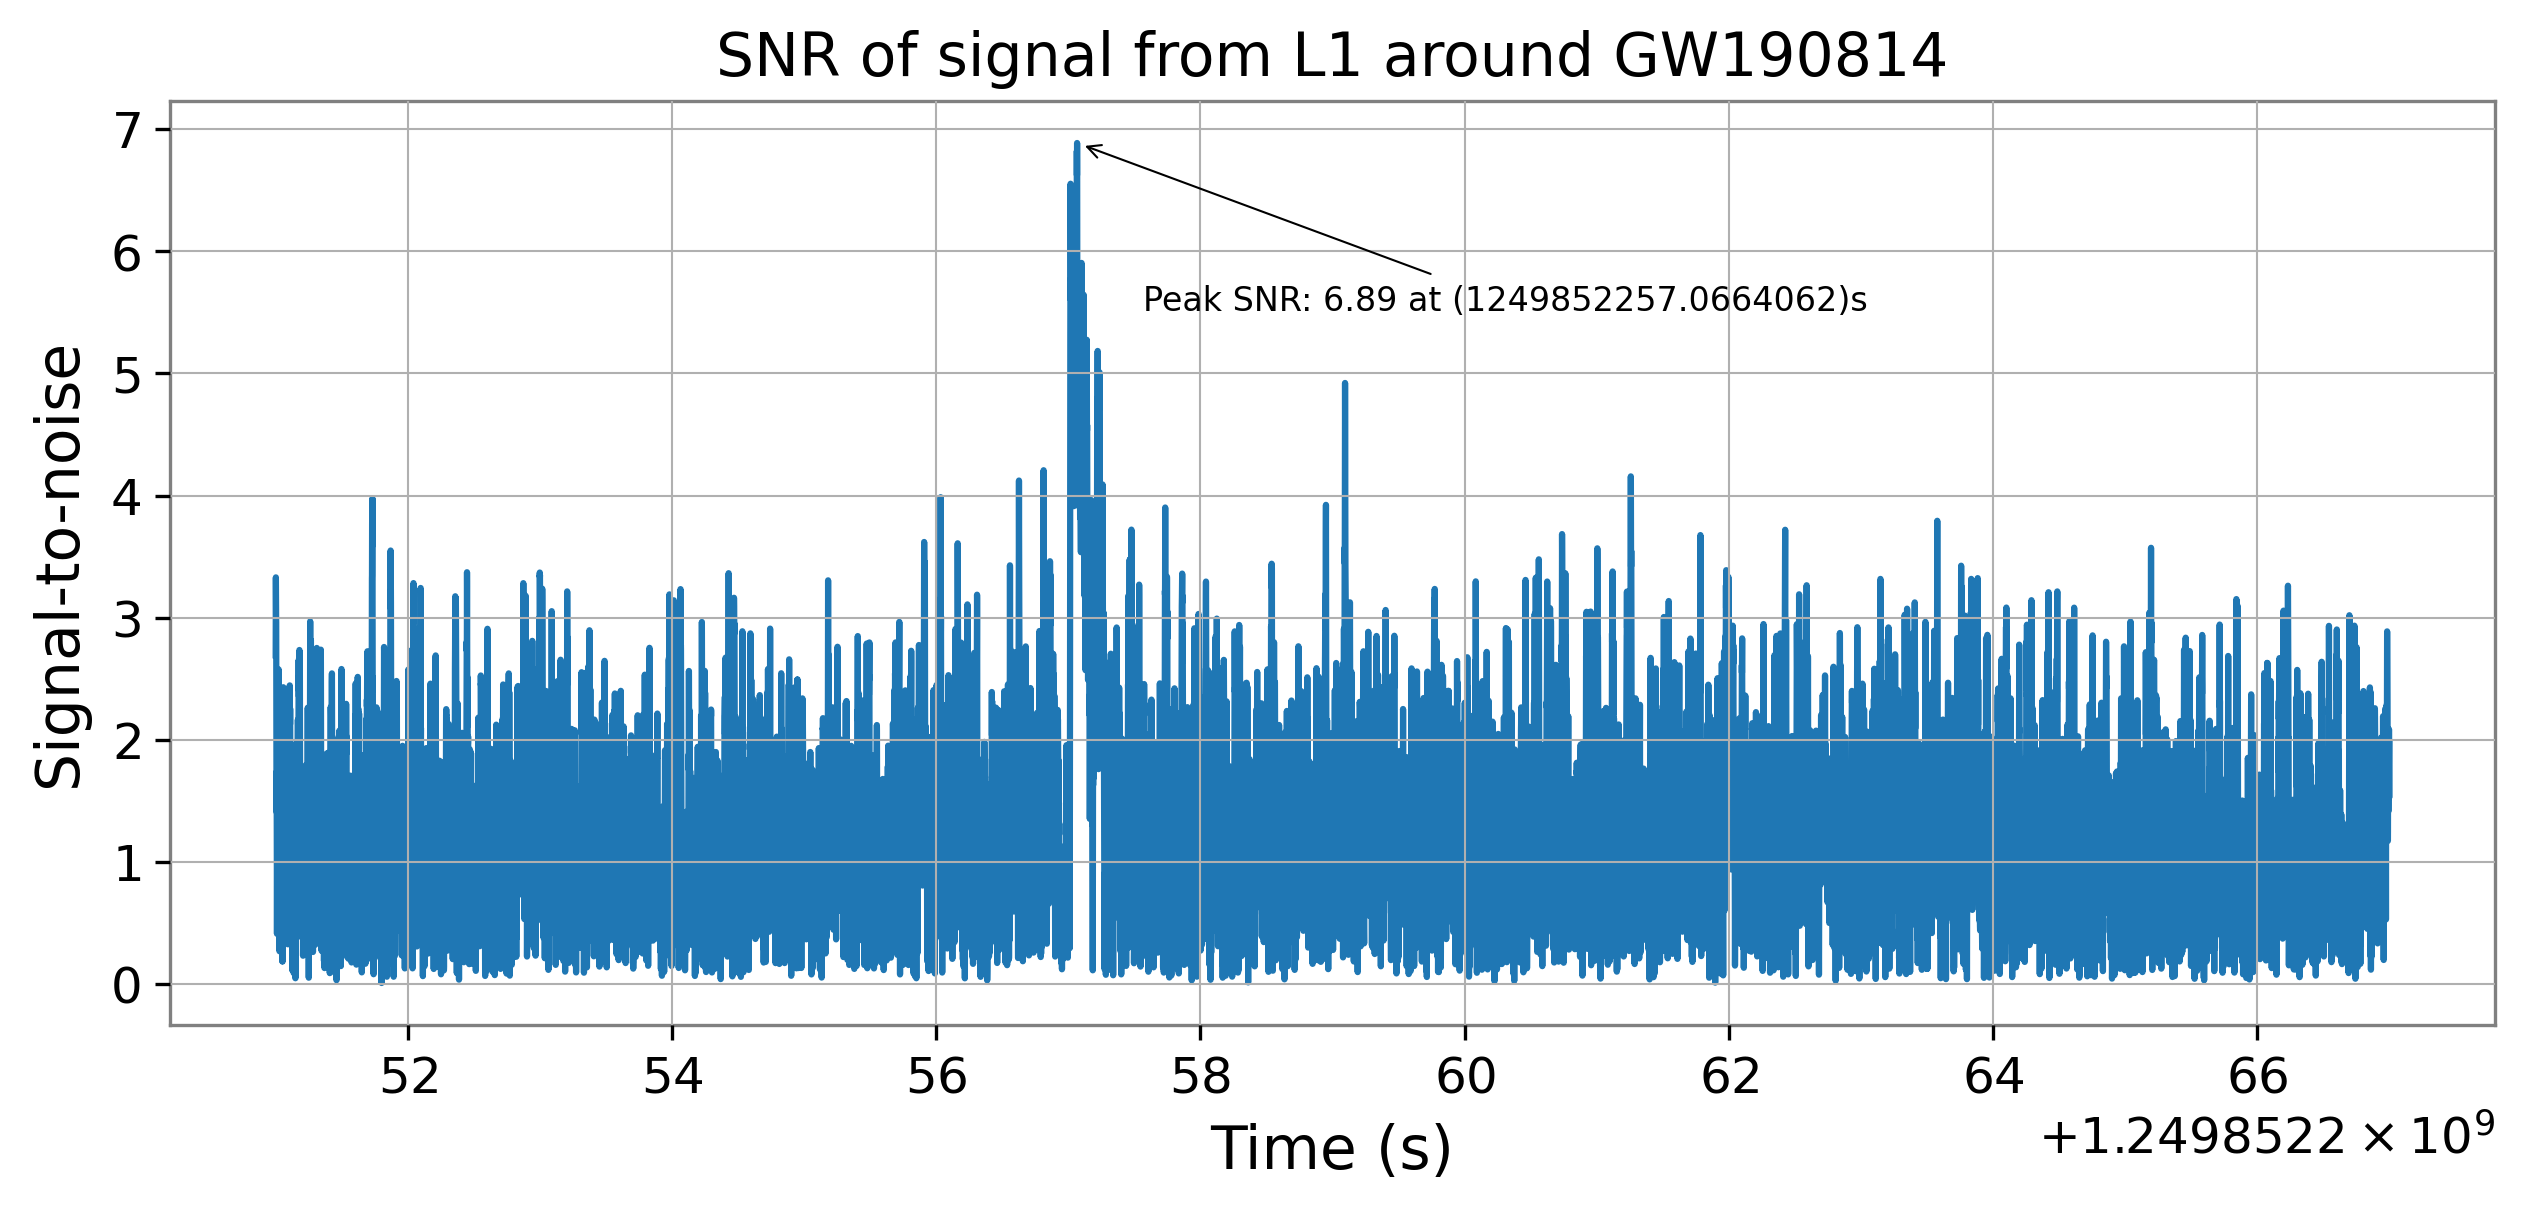
\includegraphics[width=0.75\textwidth]{GWanalysisProject_codefile/SNRplot/SNRL1GW190814.png}
%             \caption{SNR from L1 detector around GW190814}
%             \label{fig:GW190814SNR}
% \end{figure}

Similarly, the plot of the Signal-to-Noise Ratio for the signal detected by the L1 detector during incident GW190814 reveals a maximum SNR of 6.89 (Fig: \ref{fig:GW190814SNR}) at roughly 1249852257.0664062 seconds. The signal-to-noise ratio reaches its maximum value at around 58 seconds on the figure. The signal-to-noise ratio achieves an approximate maximum value of 7, confirming a robust detection of the gravitational wave event GW190814.

We generated a template plot using the \texttt{IMRPhenomPv2\_NRTidal} approximant with 2.36 $M_\odot$ for both stars and a distance of 42 Mpc, computed with a time resolution of \texttt{conditioned.delta\_t} and a 60 Hz lower frequency bound. The plot (Fig: \ref{fig:GW190814template}) shows a strong fit between the experimental data and the numerical waveform, validating Einstein's Theory of General Relativity.

% \begin{figure}[h]
%             \centering          
%             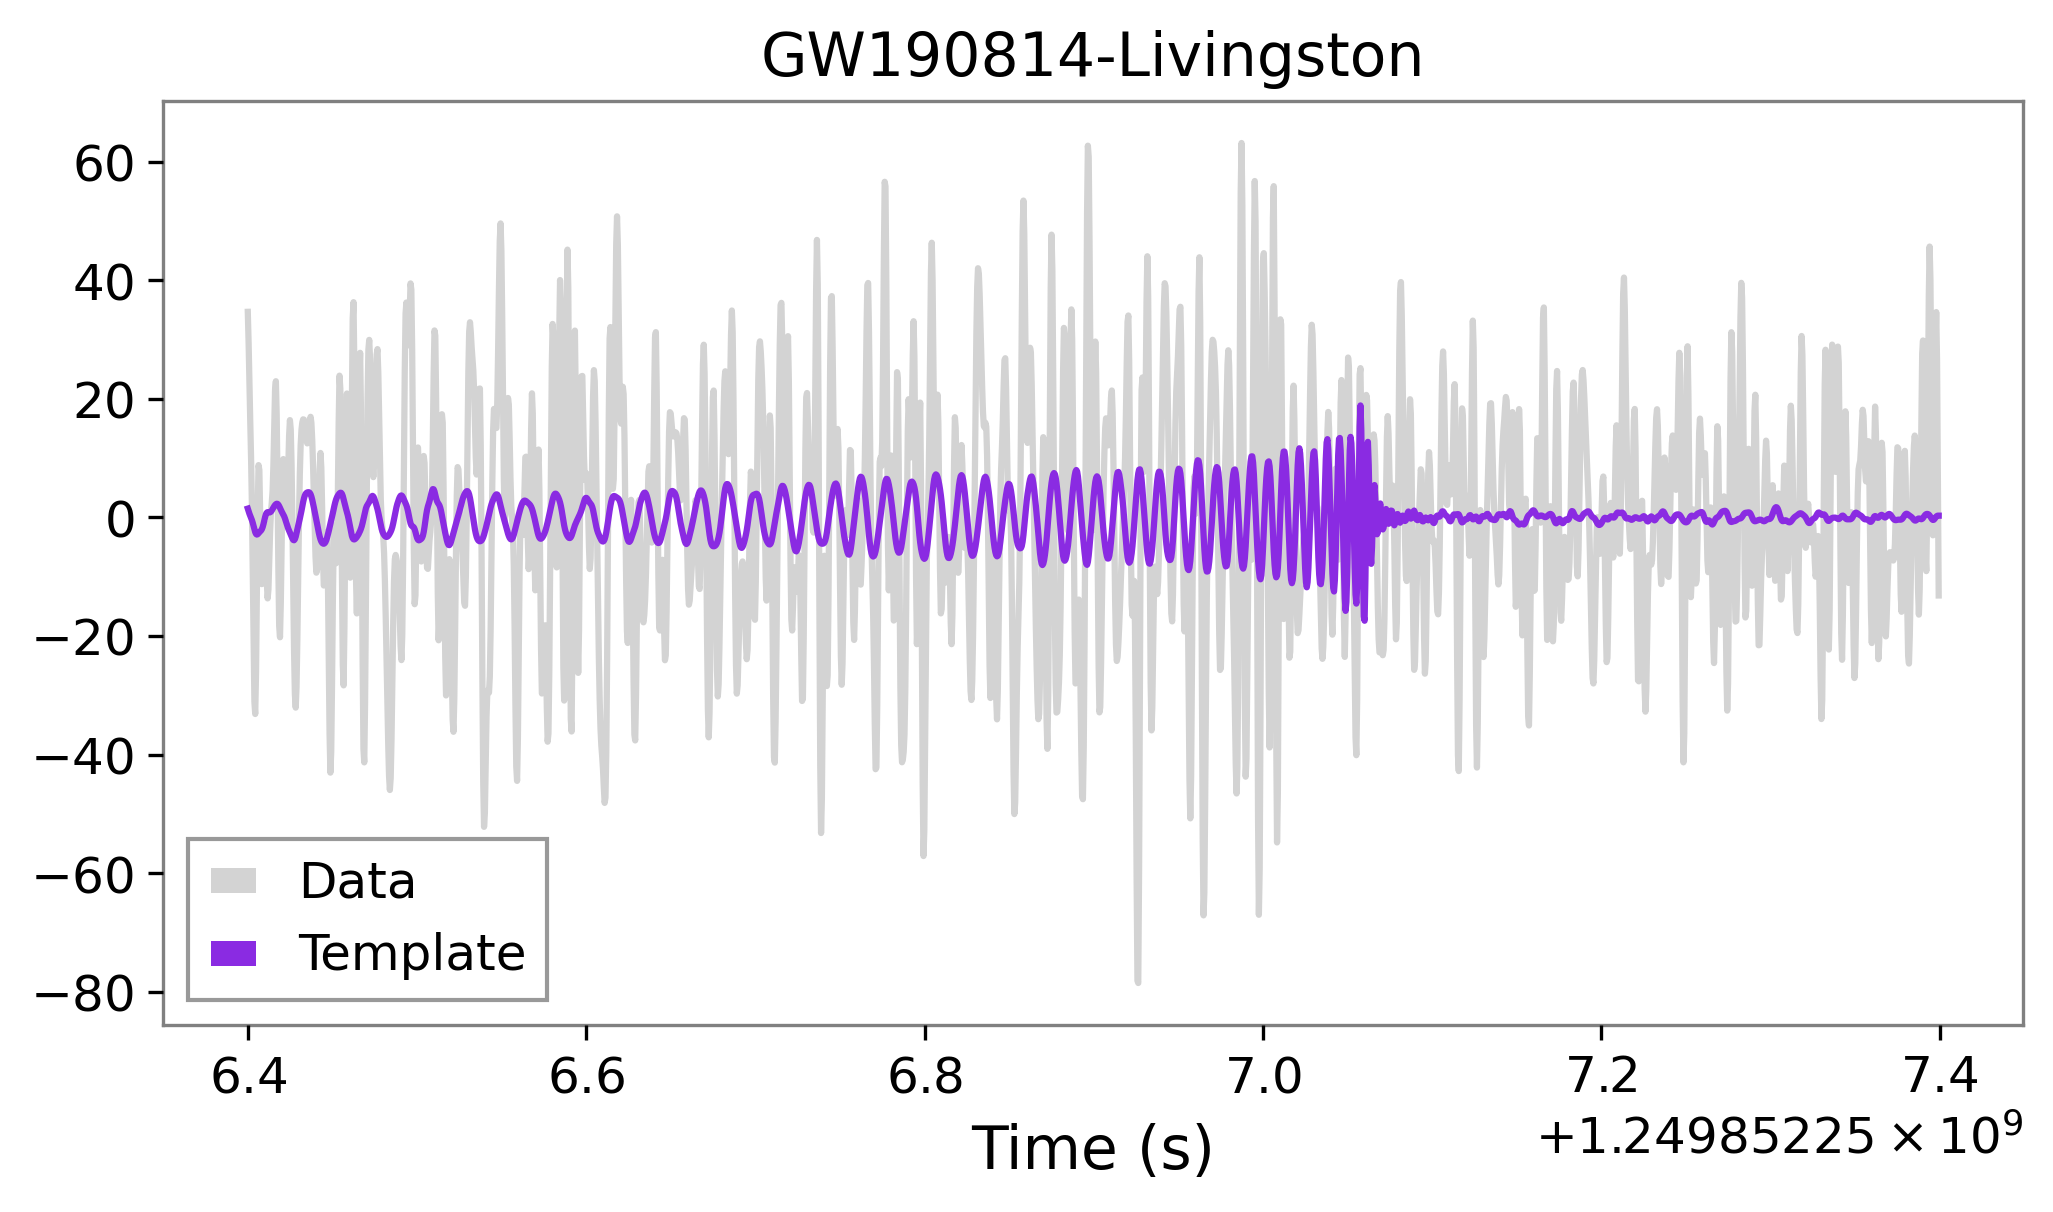
\includegraphics[width=0.75\textwidth]{GWanalysisProject_codefile/templateplot/templateL1GW190814.png}
%             \caption{Whitened Template data calculated from numerical solution of GR and actual recorded data around GW190814}
%             \label{fig:GW190814template}
% \end{figure}

Based on the comparison of gravitational wave events, including GW170817, GW190521, and GW190814, some differences and similarities between the data and the detector responses are noted. For strain data, GW170817 presents a clear chirp signal with the more prominent of the two peaks in the LIGO-Livingston data and a less noticeable chirp in the LIGO-Hanford data. On the other hand, GW190521 is characterised by relatively short and low-frequency signal mainly detected in LIGO-Livingston and LIGO-Hanford data, due to the massive black holes involved. Likewise, GW190814 has a strong chirp in LIGO-Livingston but is relatively weak in Hanford and VIRGO data. The ASD shows that LIGO-Livingston has a higher sensitivity with low strain noise than LIGO-Hanford and VIRGO for all the events detected. Higher strain noise and clear peaks at different frequencies can be observed for VIRGO which could be a sign of narrower noise sources. Further substantiation of these facts is provided by the Q-transform analysis, which indicates that GW170817 and GW190814 are characterized by distinct chirp signals in the LIGO-Livingston data, while GW190521 demonstrates a brief low-frequency signal. The Signal-to-Noise Ratio plots indicate that GW190521 and GW190814 were robustly detected, with maximum SNR values of 8.95 and 7, respectively, suggesting significant gravitational wave signals. The matching of the template fits confirms that the observed experimental results are in good agreement with the theoretical calculations based on the General Theory of Relativity by Albert Einstein.


